\section{Engineering analysis}\label{sec:analysis}

Every simulation answers one design question and ends in a design decision. Each model was checked against an analytic or published case before its results were used; the checks are collected in one box per part. Everything can be rerun from \repo{sim/acoustics/run_all.sh} and \repo{sim/spice/run_all.sh}. The full write-ups are \repo{sim/acoustics/README.md} and \repo{sim/spice/README.md}.

\begin{table}[htbp]
\centering\small
\caption{The simulations at a glance.}
\label{tab:sim-summary}
\begin{tabularx}{\linewidth}{@{}l >{\raggedright\arraybackslash}p{0.33\linewidth} >{\raggedright\arraybackslash}X@{}}
\toprule
ID & Question & Outcome \\
\midrule
A1 & PR tuning, bass limits, bass EQ & \qty{3.5}{\gram} per PR, $f_b=\qty{53}{\hertz}$; $F_3$ \qty{63.7}{\hertz}; \qty{90.6}{\decibel} pink; no zeolite \\
A2 & Tweeter bezel or waveguide? & Keep the \qty{3}{\milli\metre} bezel; the desk, not the bezel, is the problem \\
A3 & Woofer baffle step, tunnel & Smooth \qty{-5.6}{\decibel} step, cancelled by the desk; keep the tunnel (+3--\qty{4}{\decibel} horn bump) \\
A4 & Panel modes of the printed shell & Output $\ge\qty{23}{\decibel}$ below the woofers; add a spine plate and damping \\
A5 & Crossover and system EQ & LR4 at \qty{2.5}{\kilo\hertz}, tweeter \qty{-9.7}{\decibel}, \qty{+110}{\micro\second}; 7-biquad EQ \\
S1/S7 & Boost loop, start-up, rail impedance & Stable but soft at \qty{150}{\hertz}; start-up windup $\to$ ECO-001 \#1, \#2 \\
S2 & Class-D filter into real drivers & Tweeter limiter mandatory; \qty{+2}{\decibel} tweeter shelf \\
S3--S5 & NTC window, PVDD trim, ESP32 reset & \qtyrange{2.0}{60.8}{\degreeCelsius}; trim settles in $\le\qty{150}{\milli\second}$; EN capacitor \qty{2.2}{\micro\farad} \\
S6 & Flat-cable signal integrity & \qty{68}{\ohm} source resistors; \qty{53}{\mega\hertz} max SPI \\
\bottomrule
\end{tabularx}
\end{table}

% =====================================================================
\subsection{Acoustics}

The acoustic results are referenced to a \emph{seated listener}: the speaker stands on a desk, and the listener's ears are \qty{1.0}{\metre} in front of it and \qty{0.40}{\metre} above the desk top, which puts them \ang{21} below the tweeter axis. A grid of 15 seats around that point gives a ``listening-window'' average \src{sim/acoustics/README.md}.

\subsubsection{A1: Bass system (lumped model)}\label{sec:a1}

A Thiele/Small model puts two ND65-8 woofers and two DMA58-PRs in one \qty{0.82}{\litre} box. The amplifier enters as limits, not as a fixed power: a \qty{15.5}{\volt} woofer limiter (about \qty{15}{\watt}) and \qty{4.5}{\ampere} of current. The maximum output at each frequency is the lowest of four limits: amplifier voltage, amplifier current, woofer $X_\text{max}$ and PR excursion.

\textbf{Result.}
\begin{itemize}
  \item With \qty{3.5}{\gram} of washers per PR, the box tunes to \qty{53.2}{\hertz}.
  \item A four-biquad bass EQ (at most \qty{+8.8}{\decibel}) gives $F_3/F_6 = \qtylist{63.7;55.3}{\hertz}$.
  \item The pink-noise maximum is \qty{90.6}{\decibel} at \qty{1}{\metre} in half space, limited by amplifier voltage. That is only \qty{0.5}{\decibel} above the target.
\end{itemize}
Because voltage is the binding limit, stuffing and zeolite each move the result by less than \qty{0.5}{\decibel}, so zeolite was dropped. The only cheap lever is the limiter: \qty{17.1}{\volt} would add \qty{0.9}{\decibel}, at the price of overdriving the woofer's \qty{15}{\watt} rating. Both the SPL and $F_6$ margins rest on vendor T/S data, so the drivers get measured first.

\begin{figure}[htbp]
\centering
\begin{subfigure}[t]{0.49\linewidth}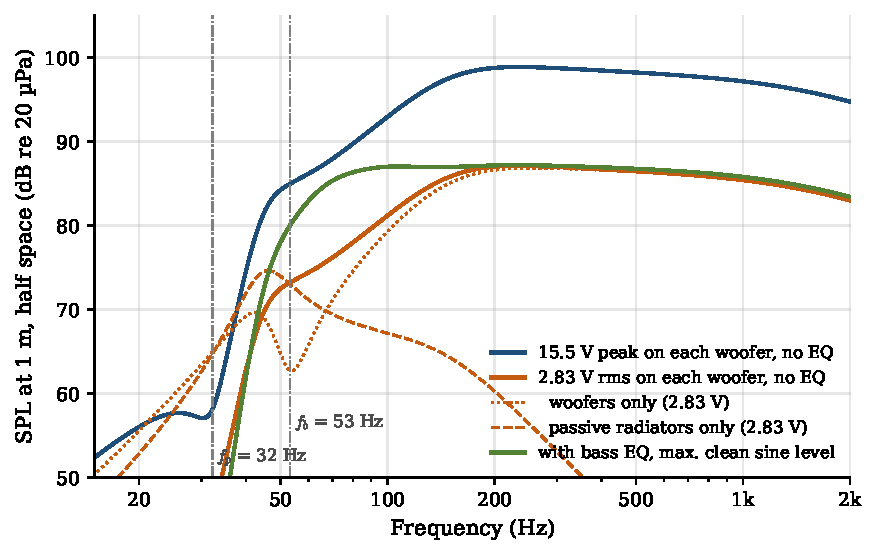
\includegraphics[width=\linewidth]{a1_spl_halfspace_1m.pdf}\caption{SPL at \qty{1}{\metre}, half space: woofer and PR contributions, full drive and the EQ'd maximum, with $f_b$ and the PR notch marked.}\end{subfigure}\hfill
\begin{subfigure}[t]{0.49\linewidth}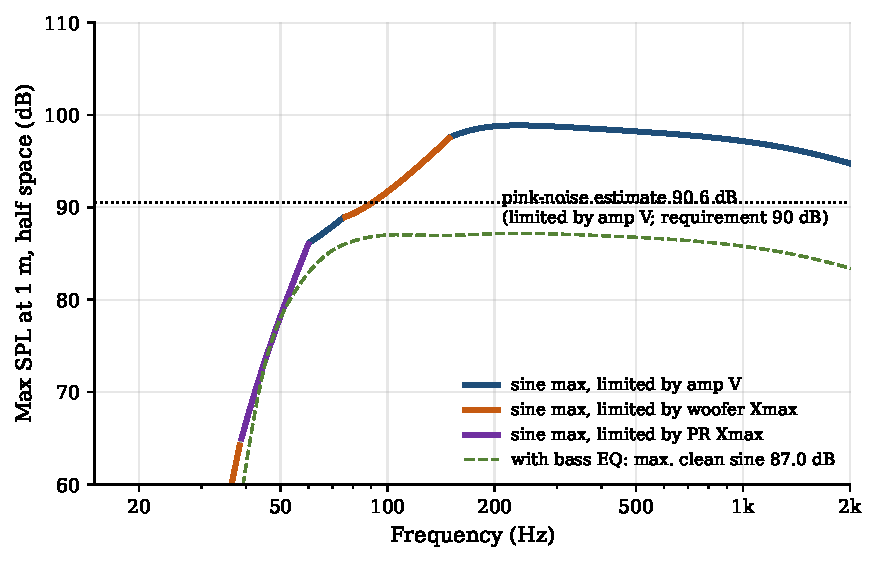
\includegraphics[width=\linewidth]{a1_max_spl_vs_frequency.pdf}\caption{Maximum sine SPL coloured by the binding limit: PR excursion below \qty{60}{\hertz}, $X_\text{max}$ from 75 to \qty{150}{\hertz}, amplifier voltage elsewhere.}\end{subfigure}\\[4pt]
\begin{subfigure}[t]{0.49\linewidth}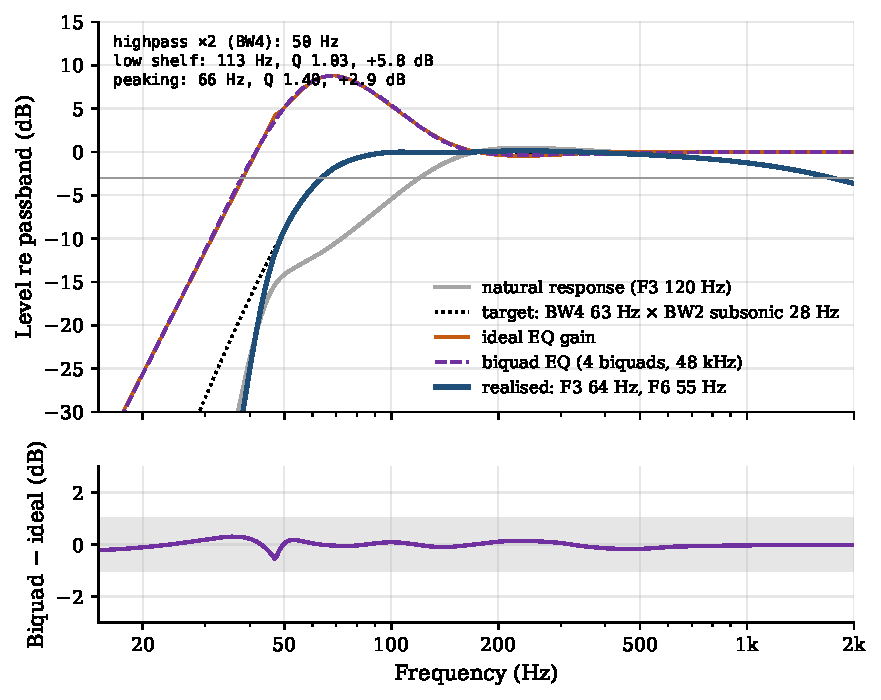
\includegraphics[width=\linewidth]{a1_dsp_bass_eq.pdf}\caption{Bass EQ: natural response, Butterworth target, 4-biquad fit (error $\le\qty{0.55}{\decibel}$).}\end{subfigure}\hfill
\begin{subfigure}[t]{0.49\linewidth}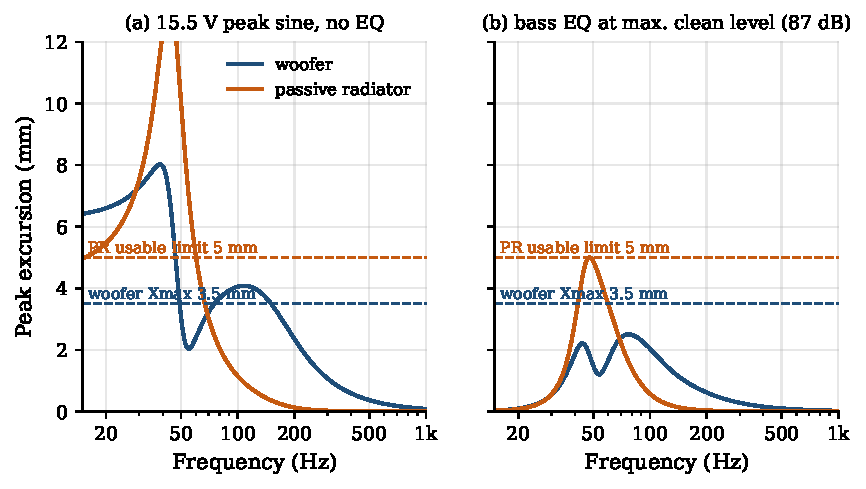
\includegraphics[width=\linewidth]{a1_excursion_vs_xmax.pdf}\caption{Excursion against limits; with EQ the PR reaches \qty{5}{\milli\metre} at \qty{48}{\hertz}, hence the subsonic roll-off.}\end{subfigure}\\[4pt]
\begin{subfigure}[t]{0.49\linewidth}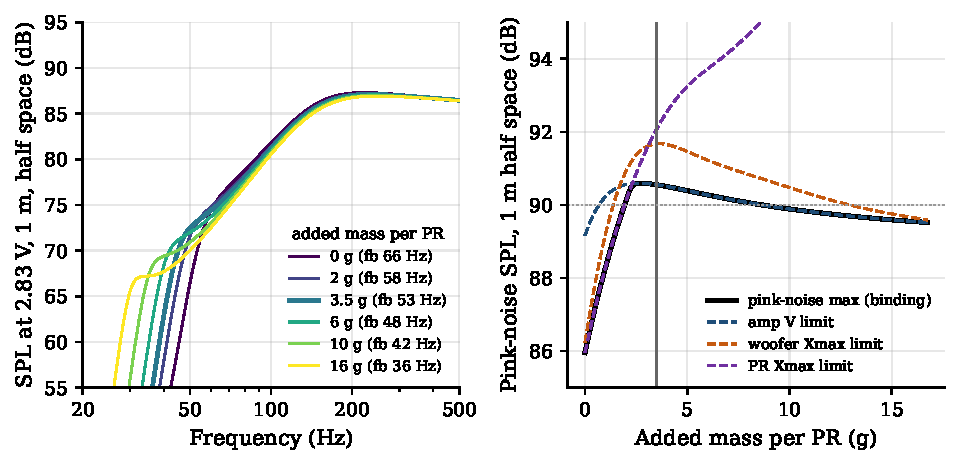
\includegraphics[width=\linewidth]{a1_pr_mass_sweep.pdf}\caption{PR mass sweep, 0--\qty{16}{\gram}: the optimum is flat from 2.5 to \qty{4}{\gram}.}\end{subfigure}\hfill
\begin{subfigure}[t]{0.49\linewidth}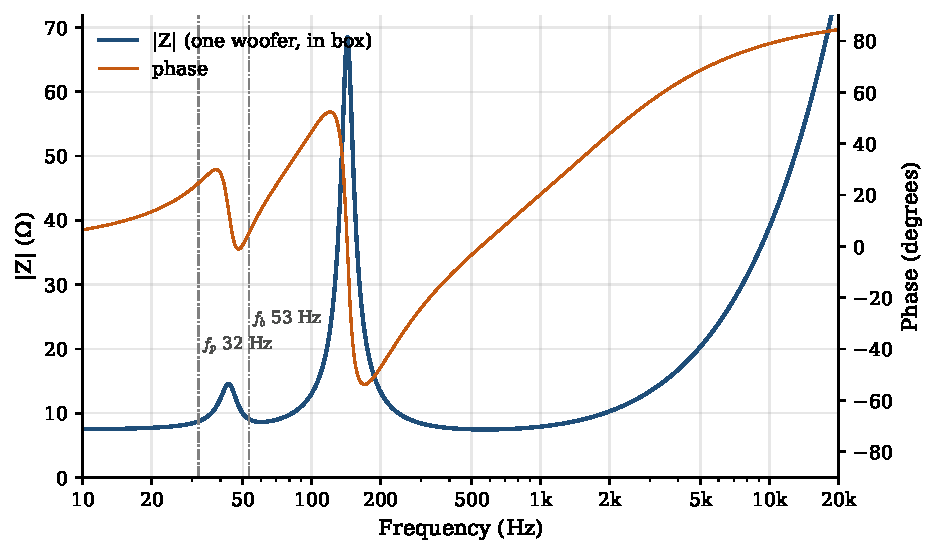
\includegraphics[width=\linewidth]{a1_impedance.pdf}\caption{Woofer impedance in the PR box: the dip near \qty{61}{\hertz} is used to tune the PRs on the bench.}\end{subfigure}
\caption{A1: the bass system. Two \qty{2.5}{inch} woofers and two passive radiators in under a litre reach \qty{64}{\hertz} with a modest DSP lift.}
\label{fig:a1}
\end{figure}

\begin{figure}[htbp]
\centering
\begin{subfigure}[t]{0.49\linewidth}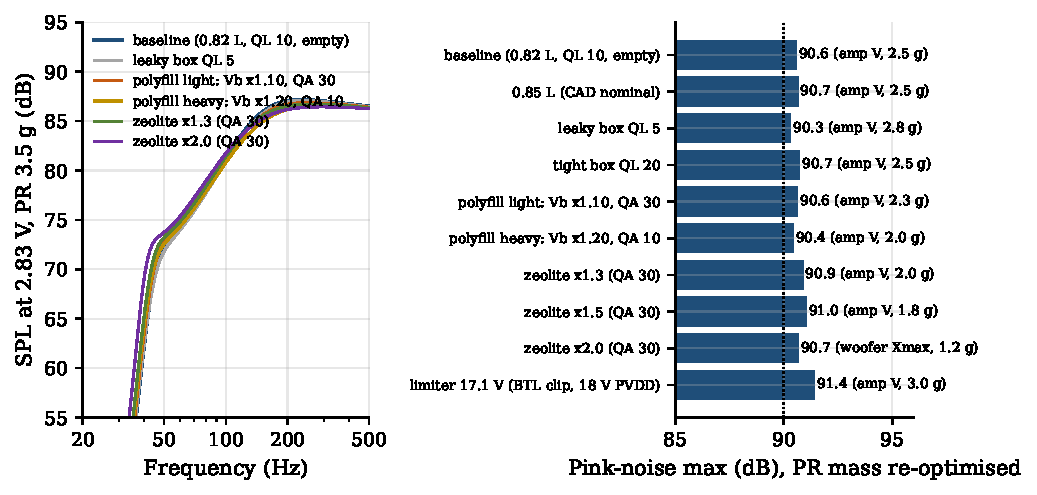
\includegraphics[width=\linewidth]{a1_whatif_volume_fill_zeolite.pdf}\caption{What-ifs: leakage, polyfill, zeolite, limiter. Only the limiter moves the pink-noise maximum by more than \qty{0.5}{\decibel}.}\end{subfigure}\hfill
\begin{subfigure}[t]{0.49\linewidth}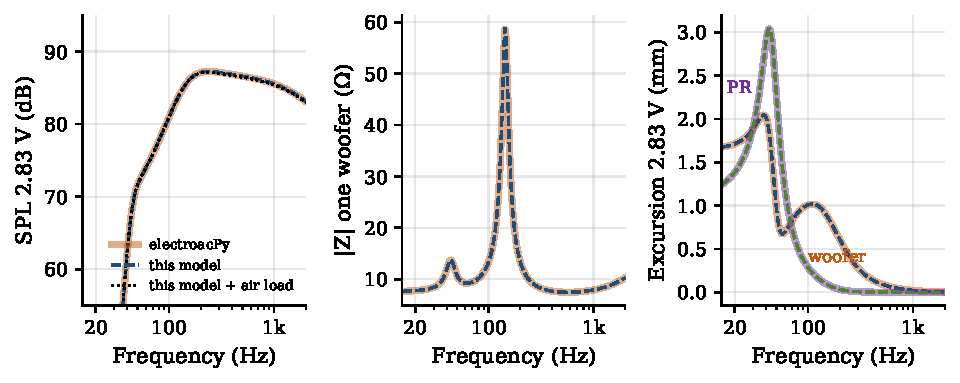
\includegraphics[width=\linewidth]{a1_electroacpy_crosscheck.pdf}\caption{Validation against electroacPy: SPL within \qty{0.013}{\decibel}, impedance within \qty{0.22}{\percent}.}\end{subfigure}\\[4pt]
\begin{subfigure}[t]{0.6\linewidth}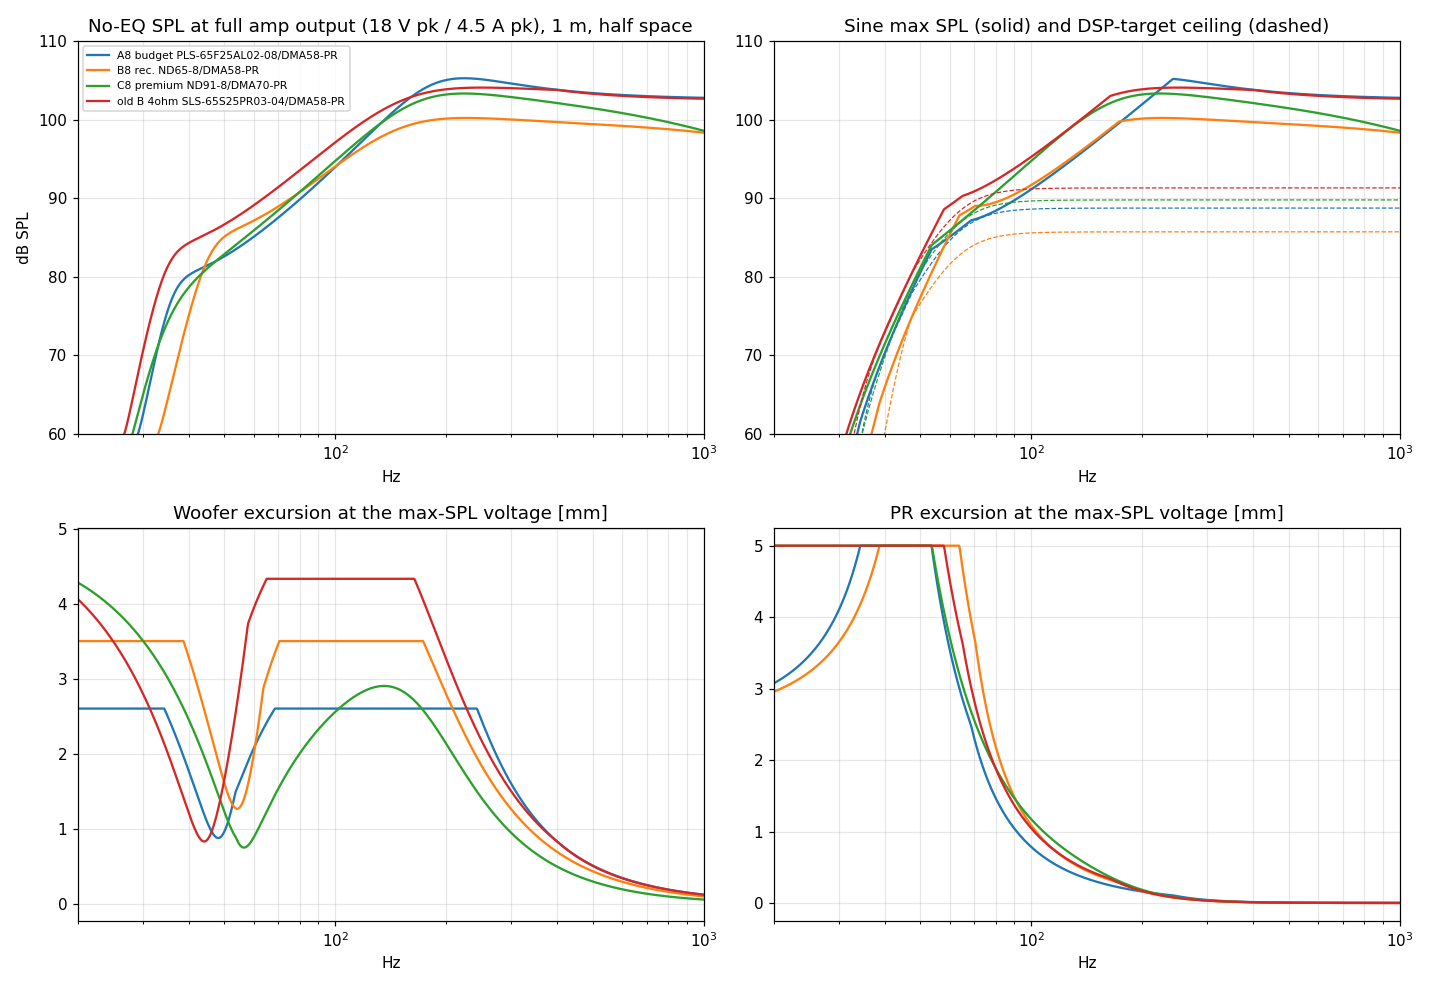
\includegraphics[width=\linewidth]{pr_alignment_firstpass.png}\caption{History: the driver agent's first-pass alignment (\qty{0.75}{\litre}, \qty{19}{\volt}), used to choose set B8.}\end{subfigure}
\caption{A1: what-ifs, validation and the first-pass model that chose the drivers.}
\label{fig:a1-more}
\end{figure}

\subsubsection{The BEM model behind A2, A3 and A5}\label{sec:bem}

The boundary-element model treats the capsule as a rigid body in free air. Each of the six radiators is a rigid piston, and bempp-cl solves the exterior problem at each of about 88 frequencies from \qty{105}{\hertz} to \qty{16}{\kilo\hertz}. Any real drive is a weighted sum of the six unit solutions. The hull is rebuilt in gmsh from the FreeCAD parameter block, so a CAD change flows straight into the acoustics. The desk is added as an image source. The meshes hold $h\le\lambda/6$, with a 9, 5.6 or \qty{3.5}{\milli\metre} global size per band and \qty{2.8}{\milli\metre} around the tweeters, giving 4\,k to 10\,k unknowns. CHIEF interior points suppress the spurious resonances of the plain formulation. The four cases run in about \qty{75}{\minute} on the laptop.

\begin{figure}[htbp]
\centering
\begin{subfigure}[t]{0.49\linewidth}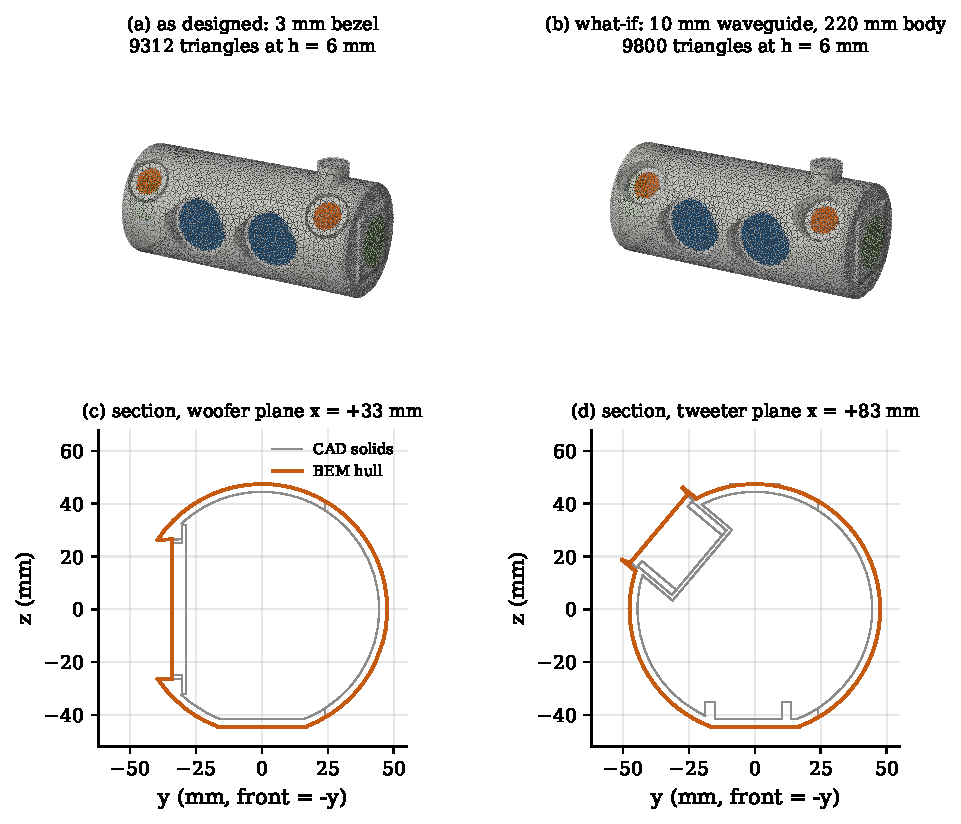
\includegraphics[width=\linewidth]{a2_a3_bem_hull_mesh_and_cad_check.pdf}\caption{Bezel and waveguide hulls with the pistons coloured, and hull sections over the CAD (median gap \qtyrange{0.7}{0.9}{\milli\metre}).}\end{subfigure}\hfill
\begin{subfigure}[t]{0.49\linewidth}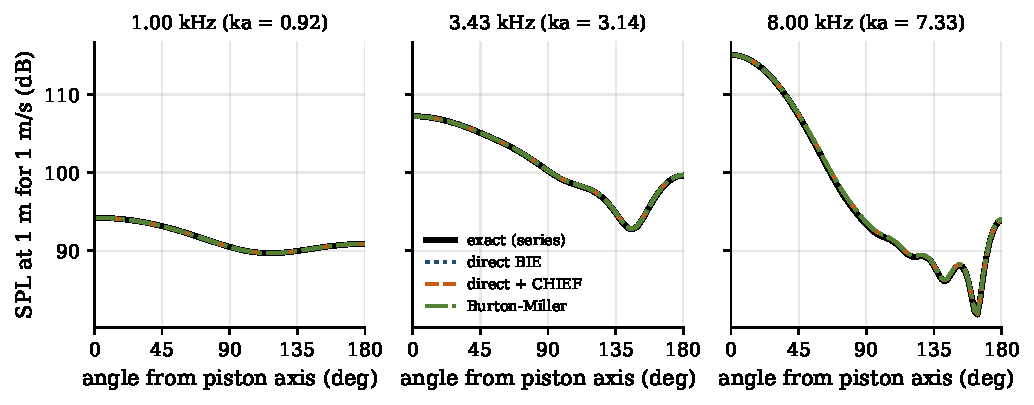
\includegraphics[width=\linewidth]{a2_a3_bem_validation_sphere_piston.pdf}\caption{Piston on a sphere against the exact solution: \qty{0.34}{\decibel} at $ka=7.3$.}\par\medskip
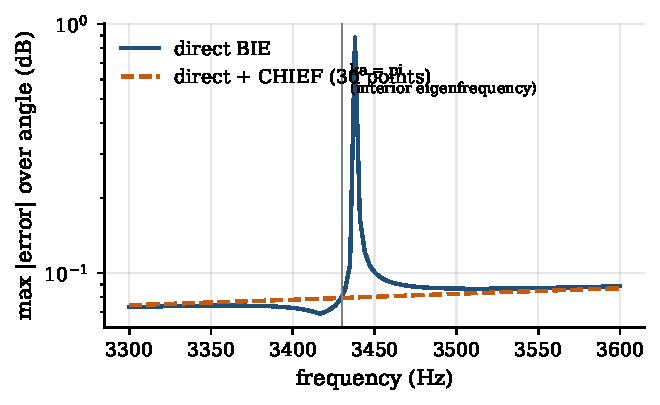
\includegraphics[width=0.8\linewidth]{a2_a3_bem_validation_irregular_frequency.pdf}\caption{Through the first interior resonance: the plain equation fails (\qty{0.88}{\decibel}); CHIEF does not.}\end{subfigure}
\caption{The BEM model and its validation.}
\label{fig:bem}
\end{figure}

\subsubsection{A2: Tweeter bezel, waveguide or flat baffle}\label{sec:a2}

\textbf{Question.} The mechanical concept had room only for a \qty{3}{\milli\metre} bezel. Would a \qty{10}{\milli\metre} waveguide, which needs a capsule about \qty{10}{\milli\metre} longer, be worth it?

\begin{table}[htbp]
\centering\small
\caption{A2: tweeter on the real capsule. Source: \protect\src{sim/acoustics/README.md}.}
\label{tab:a2}
\begin{tabular}{@{}l c c c@{}}
\toprule
 & \textbf{\qty{3}{\milli\metre} bezel} & \qty{10}{\milli\metre} waveguide & Flat baffle \\
\midrule
$-6$~dB beamwidth, horizontal, 2.5 / 5 / \qty{10}{\kilo\hertz} & \ang{310} / \ang{190} / \ang{110} & \ang{235} / \ang{128} / \ang{70} & \ang{185} \\
Directivity index, 2.5 / \qty{10}{\kilo\hertz} & 3.0 / \qty{7.9}{\decibel} & 3.8 / \qty{11.1}{\decibel} & 3.2 / \qty{6.5}{\decibel} \\
On-axis SPL, \qty{2.83}{\volt}, \qty{5}{\kilo\hertz} & \qty{87.6}{\decibel} & \qty{92.1}{\decibel} & \qty{87.3}{\decibel} \\
On-axis ripple, 2--\qty{12}{\kilo\hertz} & \textbf{\qty{2.1}{\decibel}} & \qty{4.7}{\decibel} & \qty{0.6}{\decibel} \\
Listener (\ang{21} below axis) re axis, 5 / \qty{10}{\kilo\hertz} & +0.8 / \qty{-1.8}{\decibel} & $-0.2$ / \qty{-2.6}{\decibel} & $-0.2$ / \qty{-0.8}{\decibel} \\
Desk dip, centre seat / 15-seat average & $-14.8$ / \qty{-5.6}{\decibel} & $-11.8$ / \qty{-5.3}{\decibel} & --- \\
\bottomrule
\end{tabular}
\end{table}

\textbf{Result: keep the bezel} (\cref{tab:a2}). The listener hears within \qty{2}{\decibel} of on-axis up to \qty{10}{\kilo\hertz}. The waveguide buys 3--\qty{4}{\decibel} of sensitivity, but the tweeter already runs \qty{10}{\decibel} below the woofer (A5), and this short, unoptimised flare doubles the ripple. The real treble problem is \textbf{the desk}: its reflection cancels the direct sound near \qty{2.8}{\kilo\hertz} at the centre seat (\qty{-15}{\decibel}). The dip moves with ear height, so EQ must not fill it. The physical cures are a 5--\ang{10} backward tilt on feet, or more tweeter height.

\begin{figure}[htbp]
\centering
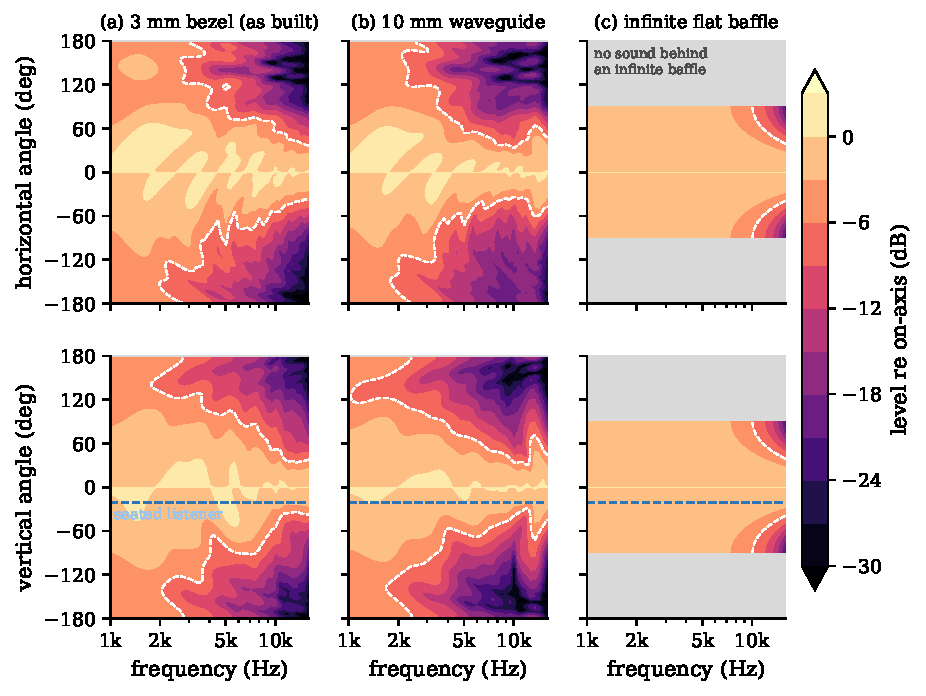
\includegraphics[width=0.8\linewidth]{a2_tweeter_polar_maps_bezel_waveguide_baffle.pdf}
\caption{A2: tweeter polar maps from 1 to \qty{16}{\kilo\hertz}, normalised to on-axis, for the bezel, the waveguide and a flat baffle. The white dashed line is \qty{-6}{\decibel}; the blue dashed line is the seated listener. The waveguide narrows the beam; the bezel behaves like a piston on a curved baffle.}
\label{fig:a2-polar}
\end{figure}

\begin{figure}[htbp]
\centering
\begin{subfigure}[t]{0.9\linewidth}\centering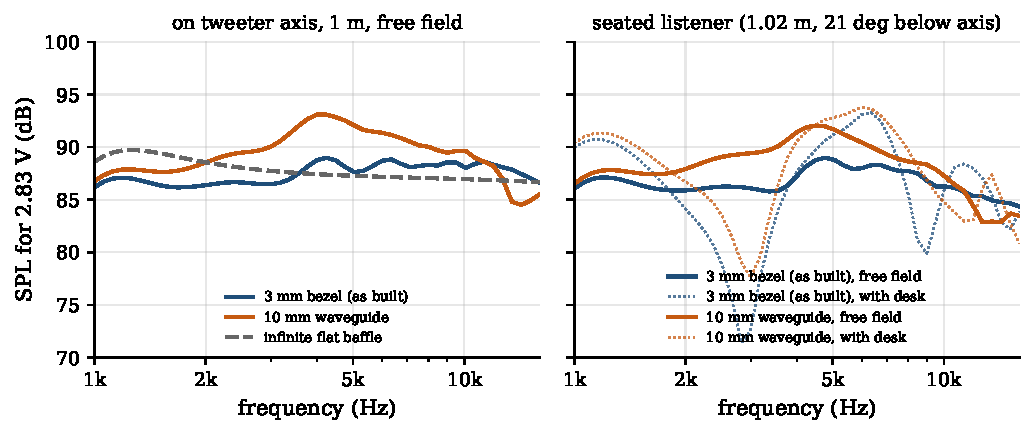
\includegraphics[width=\linewidth]{a2_tweeter_onaxis_and_listening_axis.pdf}\caption{SPL on axis and at the listener, free field and with the desk: the desk notch at \qty{2.8}{\kilo\hertz} dominates.}\end{subfigure}\\[4pt]
\begin{subfigure}[t]{0.9\linewidth}\centering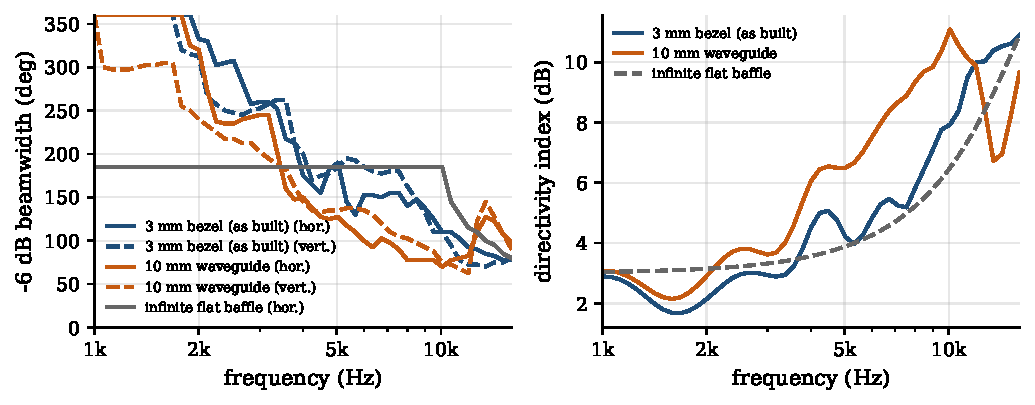
\includegraphics[width=\linewidth]{a2_tweeter_beamwidth_and_DI.pdf}\caption{$-6$~dB beamwidth and directivity index against frequency.}\end{subfigure}
\caption{A2: tweeter response and directivity.}
\label{fig:a2-resp}
\end{figure}

\subsubsection{A3: Woofer baffle step, diffraction and tunnel}\label{sec:a3}

\textbf{Question.} How large are the baffle step and the diffraction ripple on the narrow, round front? And does the \qty{14}{\milli\metre} tunnel through the baffle land matter?

\textbf{Result.}
\begin{itemize}
  \item \textbf{Baffle step.} \qty{-5.6}{\decibel} at low frequency, rising through \qty{-3}{\decibel} at \qty{643}{\hertz}. On the round front it is a smooth shelf, with only \qty{0.36}{\decibel} of ripple from \qty{150}{\hertz} to \qty{2.5}{\kilo\hertz}.
  \item \textbf{The desk gives it back.} The woofers sit \qty{44}{\milli\metre} above the desk, and the reflection adds coherently up to about \qty{2}{\kilo\hertz}. The 15-seat level rises by about \qty{5}{\decibel}, so on a desk no baffle-step boost is needed. That matters because the woofer is the voltage-limited driver. A free-standing preset would need about \qty{+5}{\decibel} below \qty{600}{\hertz}; the microphone auto-EQ can choose between the two presets.
  \item \textbf{The tunnel helps.} It acts as a short, wide horn: \qty{+3.4}{\decibel} in power at \qty{2.5}{\kilo\hertz}, peaking at \qty{+4.7}{\decibel} on axis at \qty{3.8}{\kilo\hertz}. A lumped tube model predicts the same peak height (at \qty{2.7}{\kilo\hertz}). The bump offsets the woofer's voice-coil roll-off, so the tunnel stays as designed.
  \item \textbf{Coverage.} The woofer is still wider than \ang{180} at the \qty{2.5}{\kilo\hertz} crossover.
\end{itemize}

\begin{figure}[htbp]
\centering
\begin{subfigure}[t]{0.49\linewidth}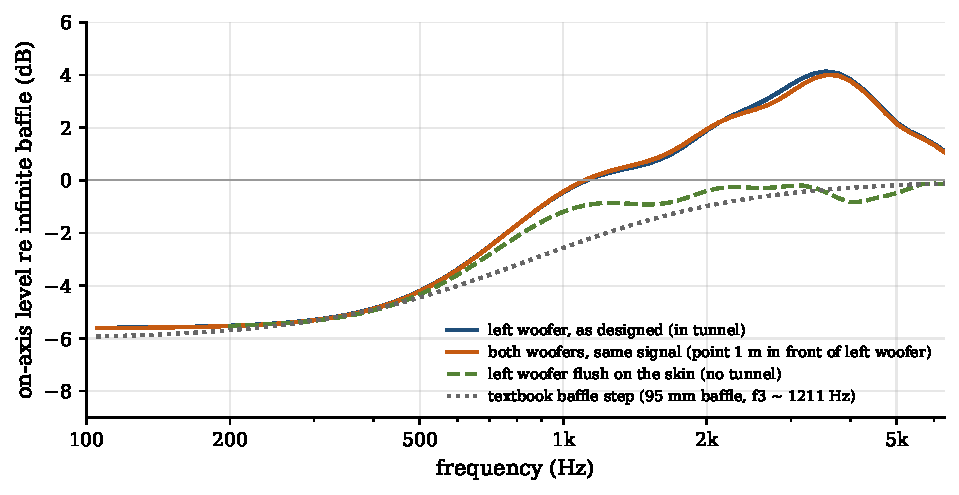
\includegraphics[width=\linewidth]{a3_woofer_baffle_step_and_diffraction.pdf}\caption{On-axis level relative to an infinite baffle: in the tunnel, both woofers, flush, and a textbook step.}\end{subfigure}\hfill
\begin{subfigure}[t]{0.49\linewidth}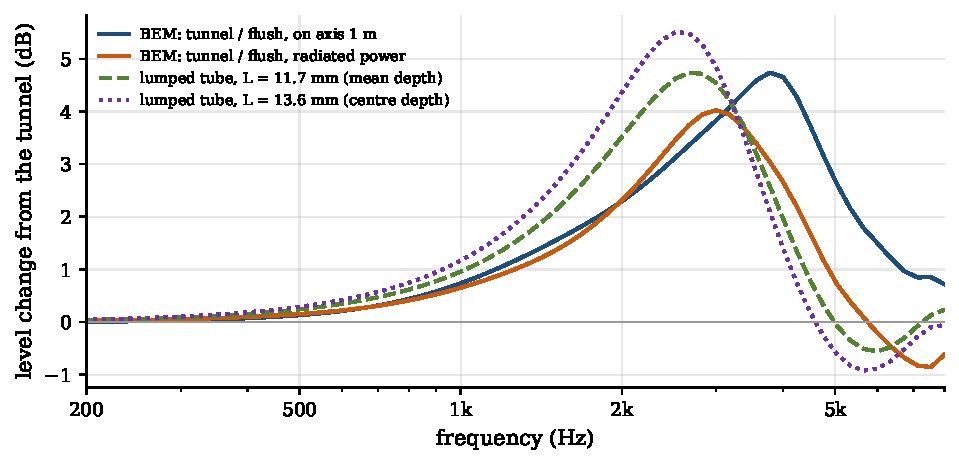
\includegraphics[width=\linewidth]{a3_woofer_tunnel_effect.pdf}\caption{Tunnel effect (BEM on axis and power) against the lumped tube model: a +3--\qty{5}{\decibel} low-Q bump.}\end{subfigure}\\[4pt]
\begin{subfigure}[t]{0.49\linewidth}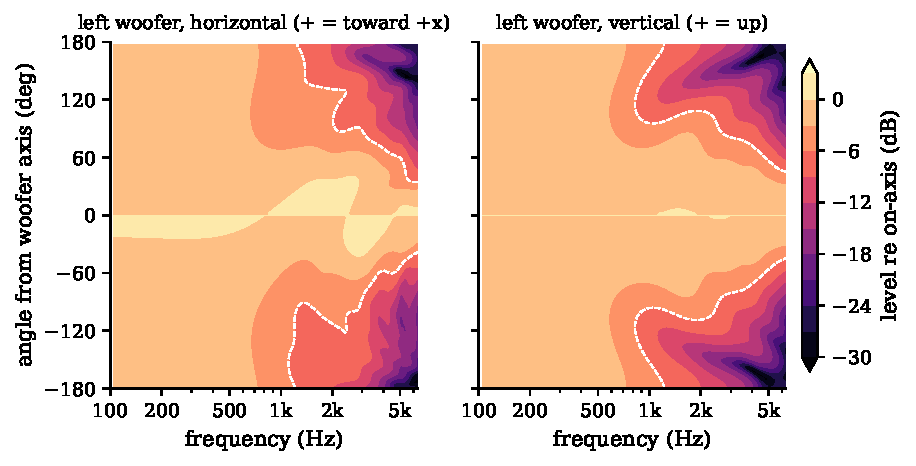
\includegraphics[width=\linewidth]{a3_woofer_polar_maps.pdf}\caption{Woofer polar maps, \qty{100}{\hertz} to \qty{6.3}{\kilo\hertz}.}\end{subfigure}\hfill
\begin{subfigure}[t]{0.49\linewidth}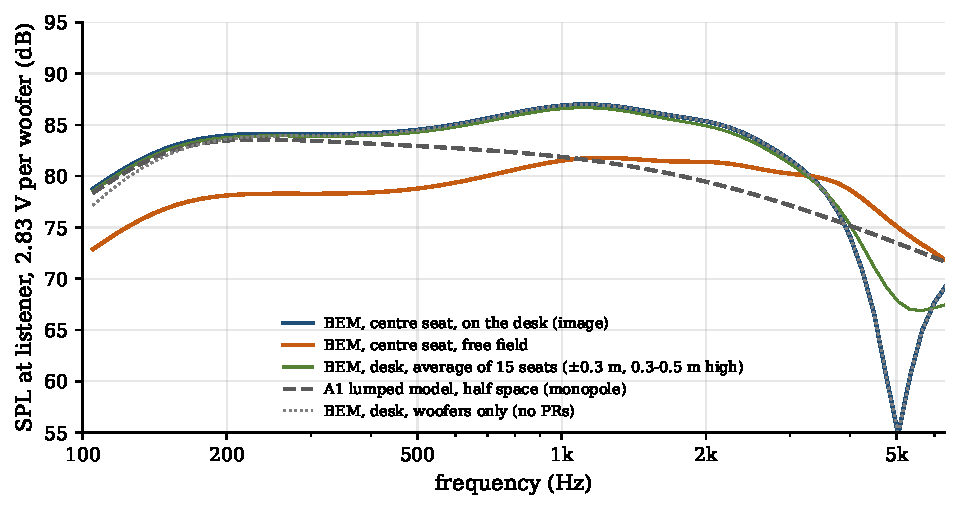
\includegraphics[width=\linewidth]{a3_woofers_and_prs_at_listener.pdf}\caption{Woofers plus PRs at the listener: on the desk, free field, 15-seat average, and A1's model.}\end{subfigure}
\caption{A3: the woofers on the real capsule.}
\label{fig:a3}
\end{figure}

\subsubsection{A4: Panel modes of the printed shell (FEM)}\label{sec:a4}

CalculiX models the five printed parts, tied together, with \qty{40}{\percent} gyroid in the thick features and the drivers and battery as lumped masses: 0.5\,M degrees of freedom, solved in \qty{2}{\minute}.

\textbf{Result.} There are 24 modes below \qty{1}{\kilo\hertz}, starting with ovalling at \qty{269}{\hertz} and a front--back squash at \qty{334}{\hertz}. Their net output stays \textbf{at least \qty{23}{\decibel} below the woofers}, which is under \qty{\pm0.5}{\decibel} of ripple. The heavy woofer frames are what keep the land quiet; without their mass the bare shell has a \qty{529}{\hertz} mode at \qty{-2}{\decibel}. The real risks are local buzz at the top (display, buttons) and a loose battery.

\textbf{Proposed bracing} (not yet in the CAD):
\begin{itemize}
  \item a \qty{1.6}{\milli\metre} centre spine plate in the \qty{2}{\milli\metre} gap between the woofers, which raises the first mode from \qty{269}{\hertz} to \qty{447}{\hertz};
  \item firm battery clamping with tray gussets;
  \item damping pads on the top and bottom flats. Raising the loss factor from 0.03 to 0.1 cuts every resonance by about \qty{10}{\decibel}, more than any rib does.
\end{itemize}

\begin{figure}[htbp]
\centering
\begin{subfigure}[t]{0.49\linewidth}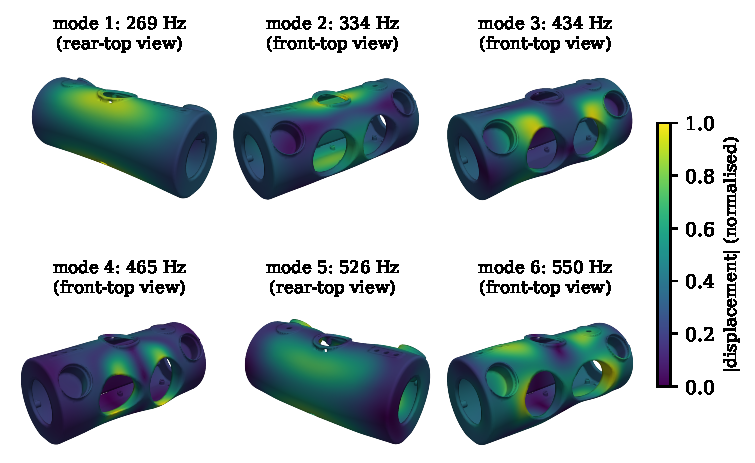
\includegraphics[width=\linewidth]{a4_mode_shapes_main_assembly.pdf}\caption{First six mode shapes: ovalling (\qty{269}{\hertz}), squash (\qty{334}{\hertz}), woofer rocking, rear shell.}\end{subfigure}\hfill
\begin{subfigure}[t]{0.49\linewidth}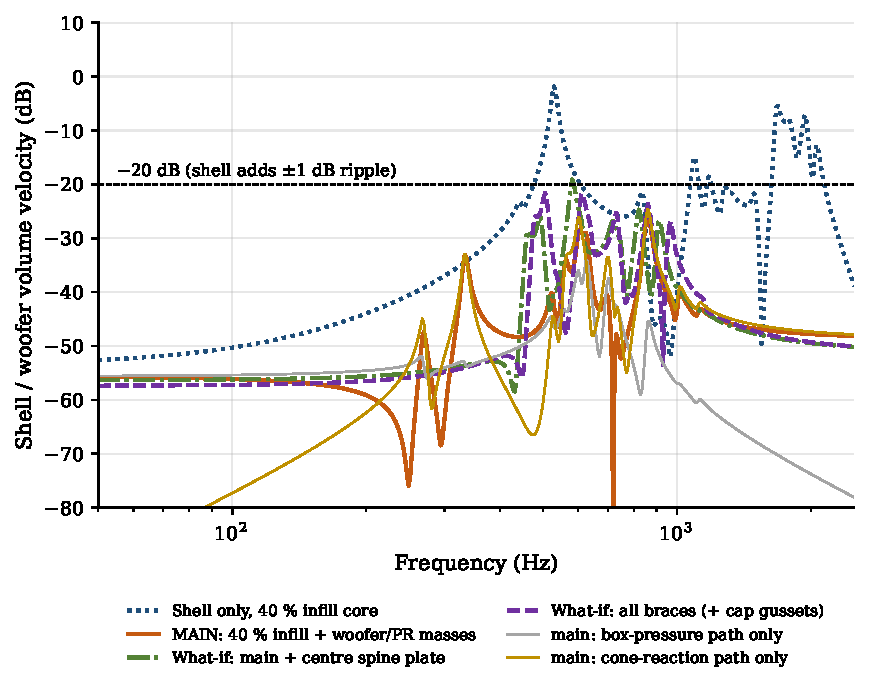
\includegraphics[width=\linewidth]{a4_shell_vs_woofer_output.pdf}\caption{Shell output relative to the woofers: bare shell, as designed, spine plate, all braces.}\end{subfigure}\\[4pt]
\begin{subfigure}[t]{0.49\linewidth}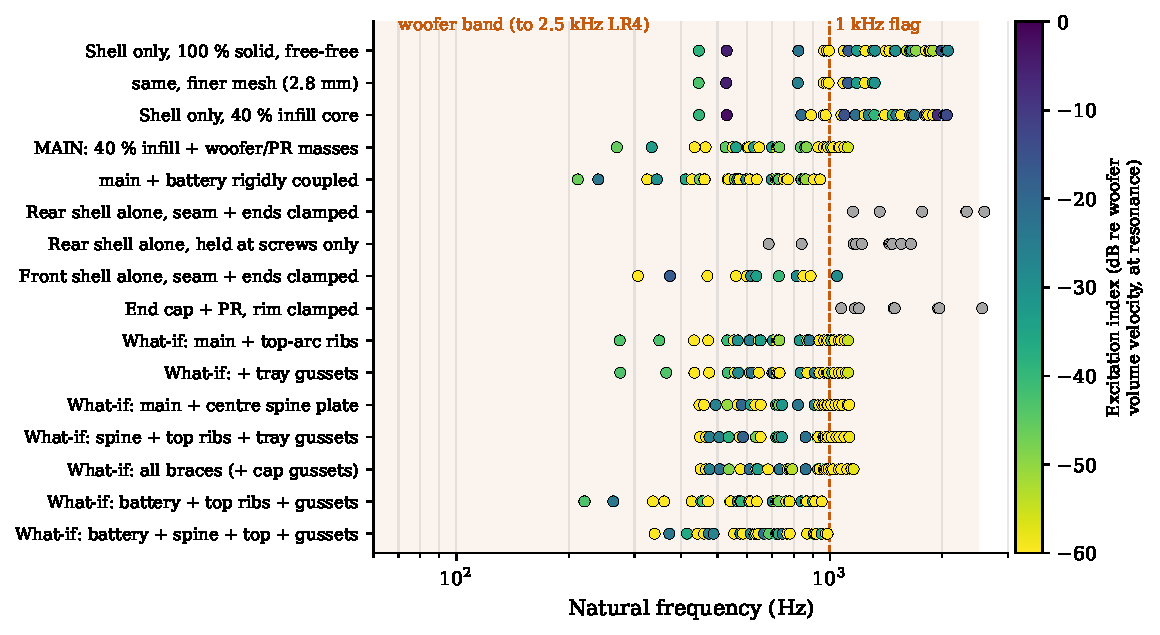
\includegraphics[width=\linewidth]{a4_modal_frequency_map.pdf}\caption{Every mode per case, coloured by how strongly the woofers drive it.}\end{subfigure}\hfill
\begin{subfigure}[t]{0.49\linewidth}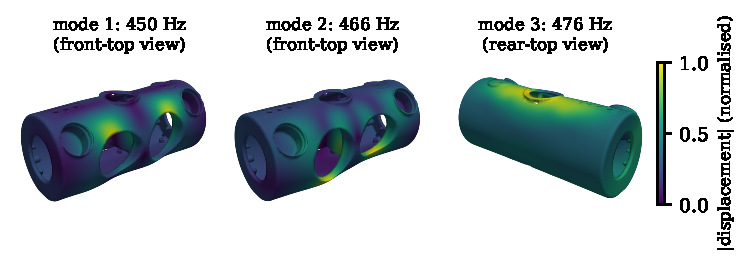
\includegraphics[width=\linewidth]{a4_mode_shapes_all_braces.pdf}\caption{With all braces the lowest mode is about \qty{450}{\hertz}.}\par\medskip
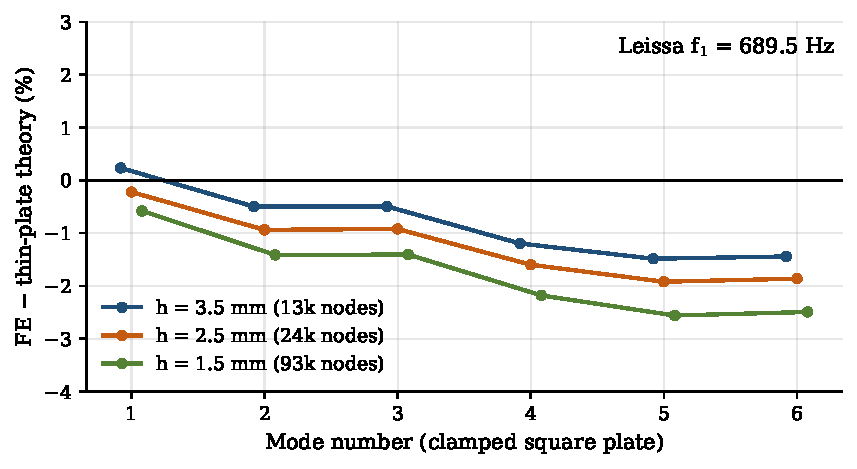
\includegraphics[width=\linewidth]{a4_validation_clamped_plate.pdf}\caption{Validation: clamped plate against Leissa, $\le\qty{1.5}{\percent}$.}\end{subfigure}
\caption{A4: panel modes of the printed enclosure.}
\label{fig:a4}
\end{figure}

\subsubsection{A5: Crossover and system EQ}\label{sec:a5}

A5 combines the A1 velocities, the tweeter model and the BEM transfer functions, with biquads at \qty{96}{\kilo\hertz}, the TAS5805M's DSP rate.

\textbf{Crossover.} LR4 at 2.0, 2.5 and \qty{3.0}{\kilo\hertz} are all well behaved: the drivers are \qty{59}{\milli\metre} apart, less than half a wavelength at \qty{2.5}{\kilo\hertz}, so no deep vertical null forms. Going lower costs tweeter excursion; going higher pushes the woofer into its tunnel bump and voice-coil roll-off. \textbf{The crossover stays at LR4, \qty{2.5}{\kilo\hertz}}, with:
\begin{itemize}
  \item the tweeter trimmed by \qty{-9.7}{\decibel}, normal polarity and delayed by \textbf{\qty{110}{\micro\second}} (11 samples at \qty{96}{\kilo\hertz});
  \item a summed response within \qty{0.05}{\decibel} rms of the ideal in-phase sum.
\end{itemize}

\textbf{System EQ.} Seven biquads were fitted to the 15-seat desk average, with cuts up to \qty{-12}{\decibel} but total boost held to about \qty{+3}{\decibel}, so the desk dip is never filled. The EQ brings the average from \qty{10.8}{\decibel} to \qty{5.0}{\decibel} peak-to-peak; what remains is mostly the desk dip. The two high-frequency filters rest on the rigid-piston model, so they must be confirmed by measurement. All filters (13 biquads on the woofer channel, 9 on the tweeter) are exported in TAS5805M 5.27 format in \repo{sim/acoustics/results/biquads_tas5805m.json}.

\begin{figure}[htbp]
\centering
\begin{subfigure}[t]{0.9\linewidth}\centering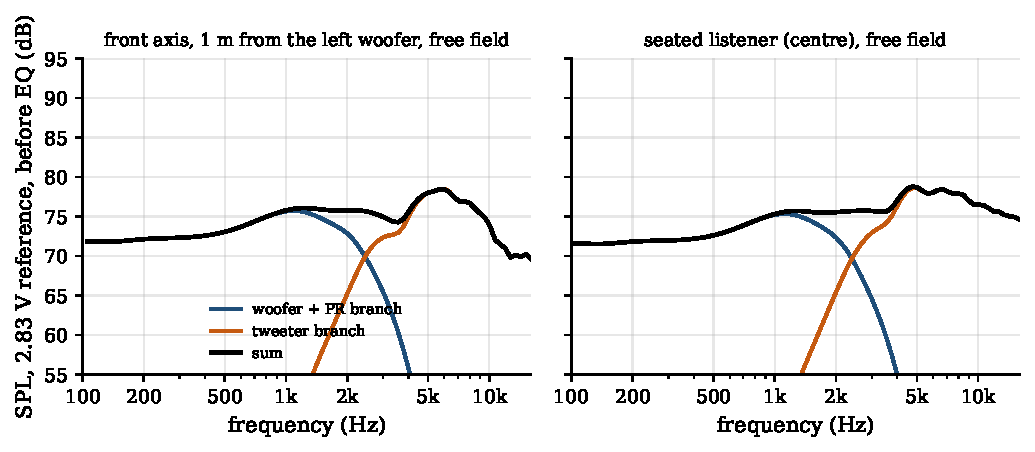
\includegraphics[width=\linewidth]{a5_crossover_branches_lr4_2k5.pdf}\caption{Woofer + PR branch, tweeter branch and sum through LR4 at \qty{2.5}{\kilo\hertz}, before EQ, on the front axis and at the seated listener.}\end{subfigure}\\[4pt]
\begin{subfigure}[t]{0.49\linewidth}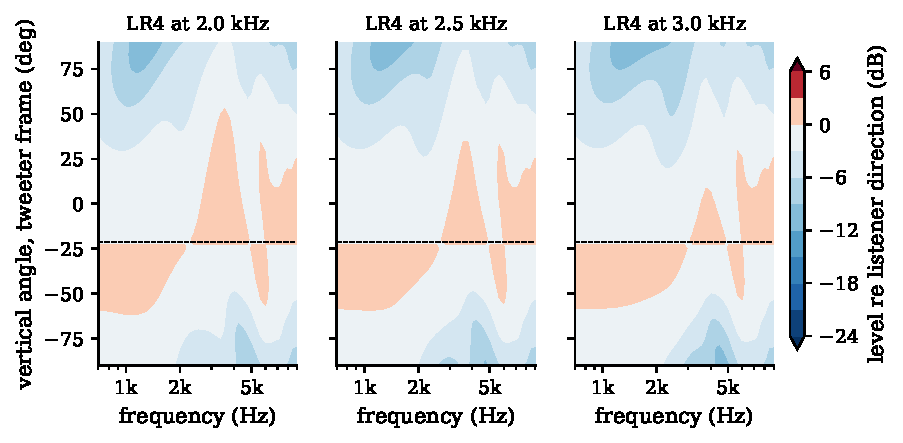
\includegraphics[width=\linewidth]{a5_vertical_lobing_vs_crossover_frequency.pdf}\caption{Vertical lobing for LR4 at 2.0, 2.5 and \qty{3.0}{\kilo\hertz}: no deep null within \ang{-50}\ldots\ang{+10} of the listener.}\end{subfigure}\hfill
\begin{subfigure}[t]{0.49\linewidth}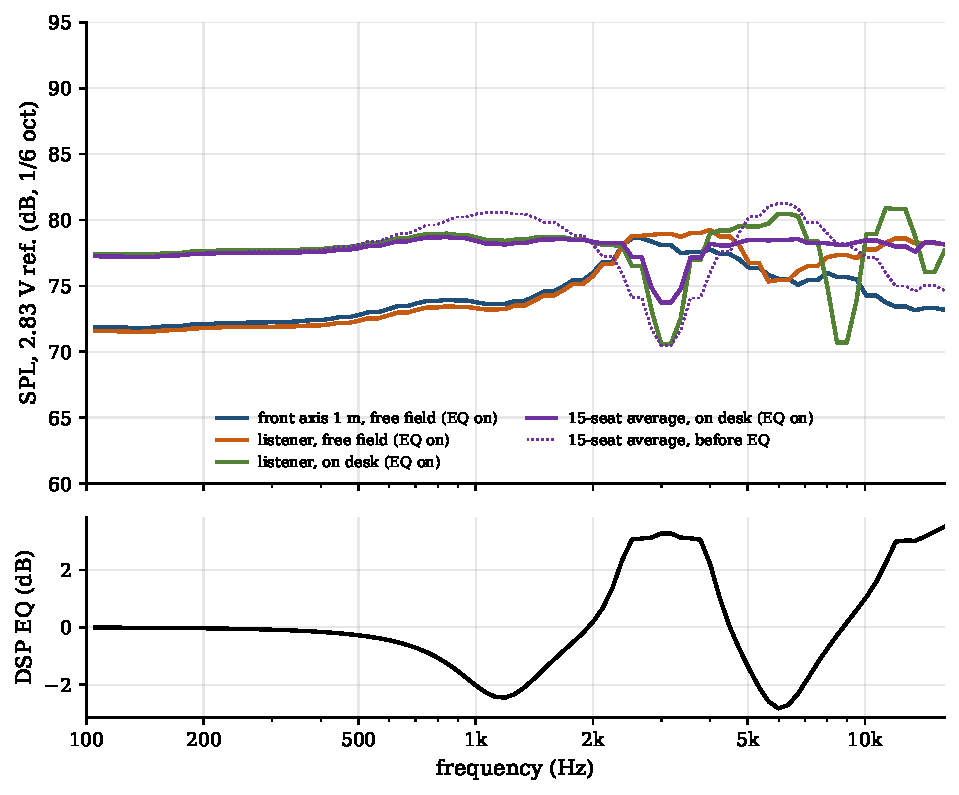
\includegraphics[width=\linewidth]{a5_system_response_per_side_with_eq.pdf}\caption{Per-side response with EQ at four positions, and the EQ curve.}\end{subfigure}\\[4pt]
\begin{subfigure}[t]{0.6\linewidth}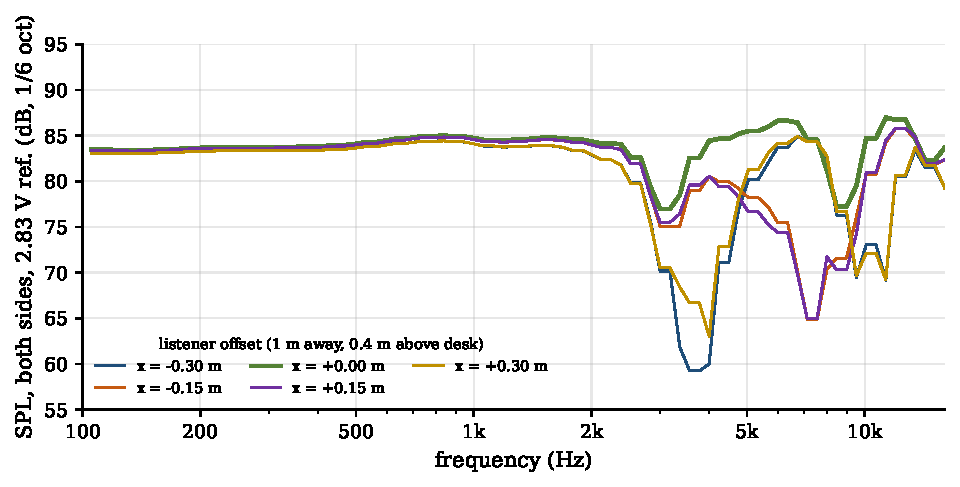
\includegraphics[width=\linewidth]{a5_stereo_pair_mono_at_seats.pdf}\caption{Both sides with a mono signal at five seats: comb filtering above \qty{3}{\kilo\hertz} off-centre, normal for any stereo pair.}\end{subfigure}
\caption{A5: crossover and system response.}
\label{fig:a5}
\end{figure}

\begin{checked}
\begin{itemize}[leftmargin=1.2em,itemsep=1pt]
  \item \textbf{A1:} the sealed-box resonance matches the closed form (\qty{140.03}{\hertz} against \qty{140.04}{\hertz}), and the model matches electroacPy within \qty{0.013}{\decibel} SPL, \qty{0.22}{\percent} impedance and \qty{0.025}{\decibel} excursion.
  \item \textbf{BEM:}
  \begin{itemize}[leftmargin=1.2em,itemsep=0pt]
    \item piston on a sphere against the exact series: \qty{0.010}{\decibel} at \qty{1}{\kilo\hertz}, \qty{0.34}{\decibel} at \qty{8}{\kilo\hertz};
    \item CHIEF against Burton--Miller on the real capsule: within \qty{0.15}{\decibel} (tweeter);
    \item \textbf{mesh convergence at \qty{5}{\kilo\hertz}:} the first, uniform mesh was off by up to \qty{1.3}{\decibel} at the tweeter. Doubling the CHIEF points did not help, which showed the error came from the mesh, so the tweeter zone was refined to \qty{2.8}{\milli\metre} and everything re-run. Production meshes are within \qty{0.3}{\decibel} of a finer reference;
    \item the BEM bass level at the listener matches A1 within \qty{0.43}{\decibel}, and left and right tweeters mirror within a median \qty{0.26}{\decibel}.
  \end{itemize}
  \item \textbf{A4:} clamped plate against Leissa within \qty{1.5}{\percent}; mesh refinement moves the first eight modes by $\le\qty{0.4}{\percent}$.
  \item \textbf{A5:} the LR4 sum is within \qty{0.05}{\decibel} of ideal; every encoded TAS5805M word decodes back within $2^{-26}$.
\end{itemize}
\end{checked}

% =====================================================================
\FloatBarrier
\subsection{Circuits and power distribution (SPICE, PDN)}\label{sec:spice}

All circuit simulations ran in ngspice and Python \src{sim/spice/README.md}. TI publishes an unencrypted transient model of the TPS61178, and it runs unmodified in ngspice.

\subsubsection{S1 and S7: the boost loop and the amplifier rail}\label{sec:s1}\label{sec:s7}

\textbf{Finding 1: stable, but soft.} The loop has at least \ang{64.8} of phase margin everywhere. With \qty{1.5}{\milli\farad} on the rail, though, it crosses over at only about \qty{250}{\hertz}. The rail impedance therefore peaks at \qtyrange{0.46}{0.57}{\ohm} near \qty{150}{\hertz}, 3.4--$4.2\times$ the \qty{0.137}{\ohm} target, exactly where bass draws current. A \qty{5}{\ampere} bass transient would sag PVDD by more than \qty{2}{\volt}. Raising $R_c$ to \qty{100}{\kilo\ohm} (ECO-001 \#1) brings the peak to \qty{0.16}{\ohm} and cuts a load-step dip from \qty{0.97}{\volt} to \qty{0.34}{\volt}, at no cost. The worst impedance on the board sits at \qty{150}{\hertz}, not at gigahertz. The +3V3 rail meets its \qty{0.30}{\ohm} target with margin.

\textbf{Finding 2: start-up windup.} The internal soft start finishes in \qty{3.2}{\milli\second}, but charging the bank takes \qty{11}{\milli\second} at the current limit. The error amplifier winds up, and PVDD overshoots to \qty{19.4}{\volt} (typical) or to the \qty{21}{\volt} OVP. A faster loop does not help. The fix is a firmware soft start through the trim network (ECO-001 \#2).

\begin{figure}[htbp]
\centering
\begin{subfigure}[t]{0.49\linewidth}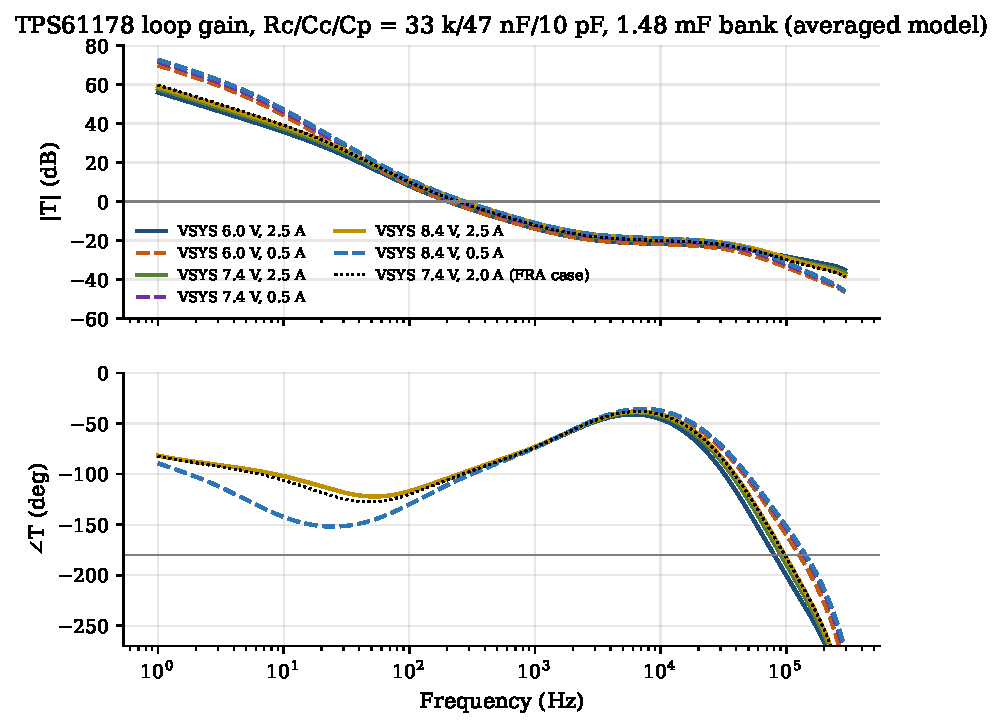
\includegraphics[width=\linewidth]{s1_loop_bode.pdf}\caption{Loop gain across input voltage and load.}\end{subfigure}\hfill
\begin{subfigure}[t]{0.49\linewidth}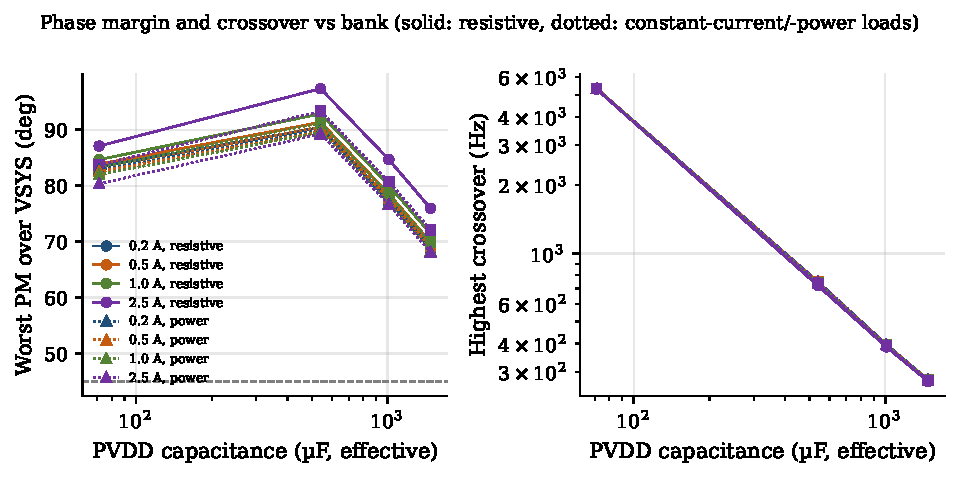
\includegraphics[width=\linewidth]{s1_loop_margins.pdf}\caption{Worst phase margin and crossover against PVDD capacitance.}\end{subfigure}\\[4pt]
\begin{subfigure}[t]{0.49\linewidth}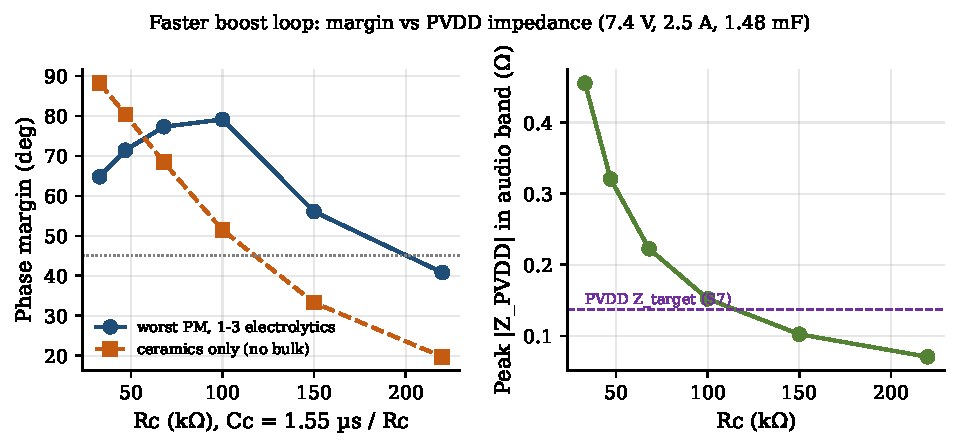
\includegraphics[width=\linewidth]{s1_compensation_options.pdf}\caption{$R_c$ sweep: \qty{100}{\kilo\ohm} reaches the impedance target with PM $\ge\ang{79}$.}\end{subfigure}\hfill
\begin{subfigure}[t]{0.49\linewidth}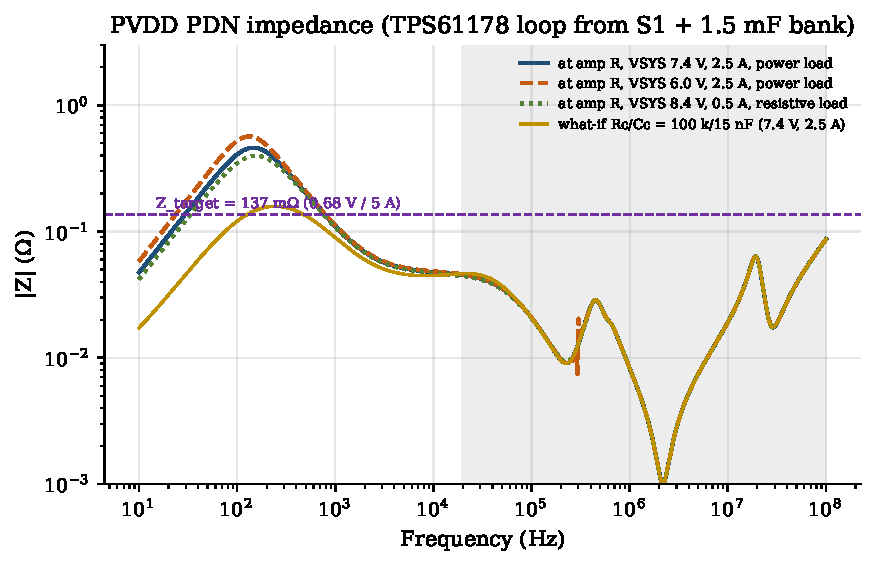
\includegraphics[width=\linewidth]{s7_pdn_pvdd.pdf}\caption{PVDD impedance at the amplifier: the \qty{150}{\hertz} peak and the ECO fix against the target.}\end{subfigure}\\[4pt]
\begin{subfigure}[t]{0.49\linewidth}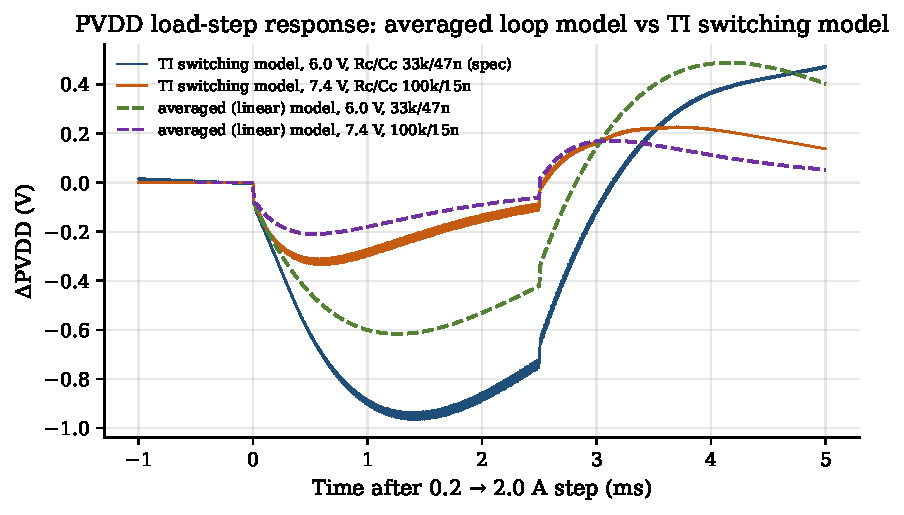
\includegraphics[width=\linewidth]{s1_loadstep.pdf}\caption{\qtyrange{0.2}{2}{\ampere} step: averaged model against TI's switching model.}\end{subfigure}\hfill
\begin{subfigure}[t]{0.49\linewidth}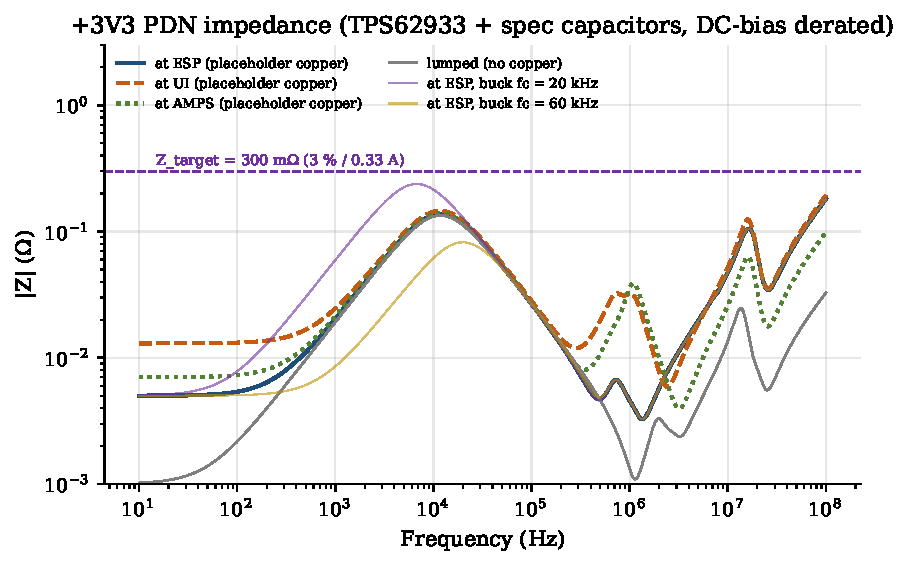
\includegraphics[width=\linewidth]{s7_pdn_3v3.pdf}\caption{+3V3 impedance: within its \qty{0.30}{\ohm} target.}\end{subfigure}
\caption{S1/S7: the boost loop and the rails. Small-signal stability is fine; the problem is impedance in the bass band.}
\label{fig:s1}
\end{figure}

\begin{figure}[htbp]
\centering
\begin{subfigure}[t]{0.49\linewidth}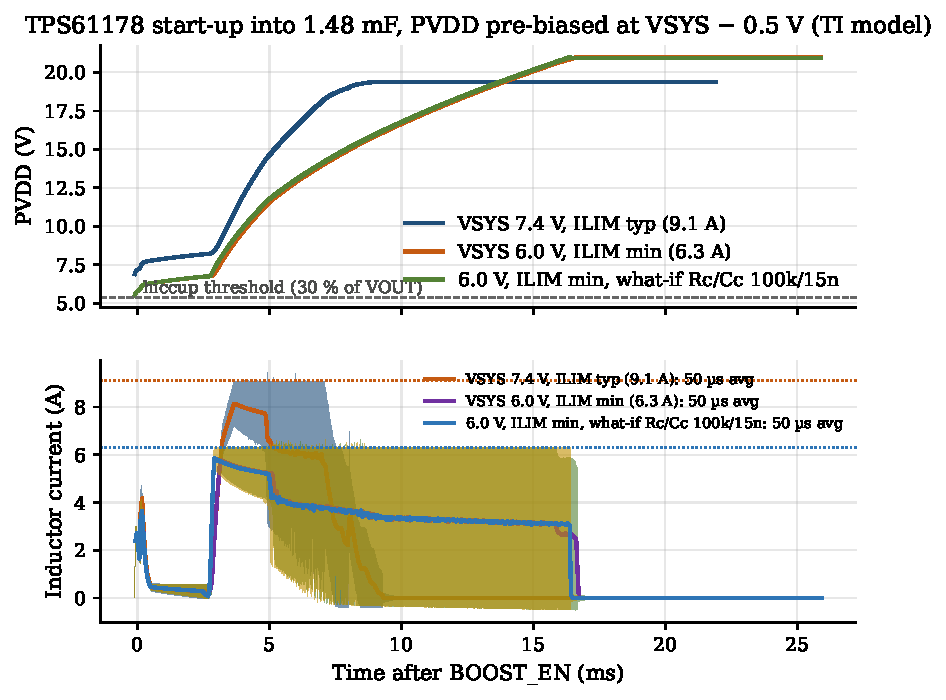
\includegraphics[width=\linewidth]{s1_startup.pdf}\caption{Start-up into \qty{1.5}{\milli\farad}: \qty{11}{\milli\second} in current limit, then overshoot from windup.}\end{subfigure}\hfill
\begin{subfigure}[t]{0.49\linewidth}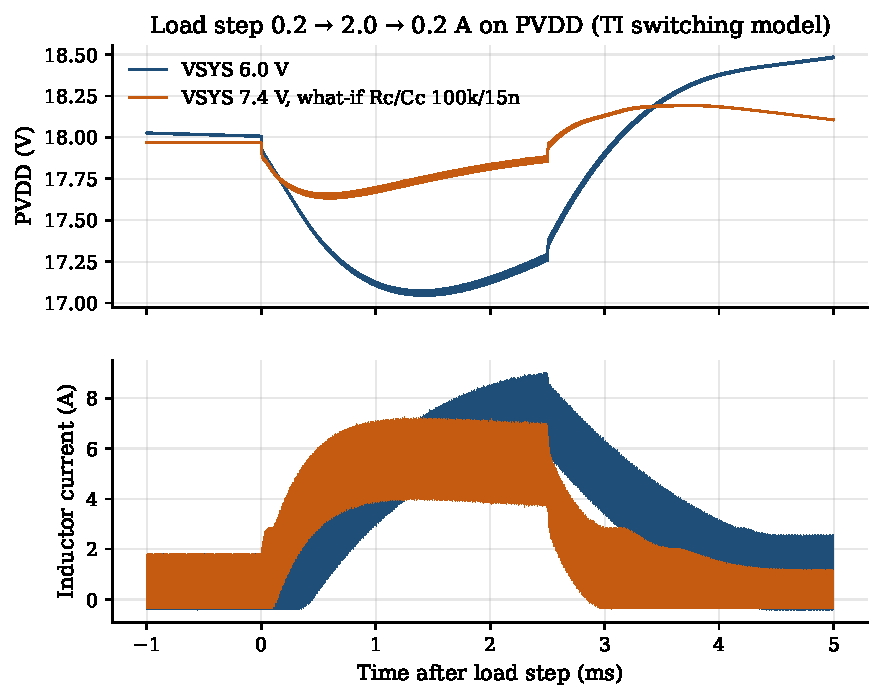
\includegraphics[width=\linewidth]{s1_loadstep_switching.pdf}\caption{Load step and release in the TI model; PFM cannot sink current, so the release overshoots.}\end{subfigure}
\caption{S1: large-signal behaviour that the datasheet equations hide.}
\label{fig:s1-large}
\end{figure}

\subsubsection{S2: Class-D output filter into the real drivers}\label{sec:s2}

Into the real tweeter impedance, the \qty{10}{\micro\henry}/\qty{1}{\micro\farad} filter droops \qty{2.2}{\decibel} by \qty{20}{\kilo\hertz}. The spec had estimated \qty{0.44}{\decibel} with a resistor load, and the fix is a \qty{+2}{\decibel} shelf (ECO-001 \#5). Into the woofer's \qty{0.61}{\milli\henry}, the filter is almost unloaded and peaks at \qty{59}{\kilo\hertz} ($Q\approx14$), which is harmless after the crossover. With the limiters, inductor current stays at or below \qty{2.7}{\ampere}. A hard-clipped tweeter reaches \qty{5.41}{\ampere}, past the \qty{5}{\ampere} trip, so the tweeter limiter is mandatory.

\begin{figure}[htbp]
\centering
\begin{subfigure}[t]{0.49\linewidth}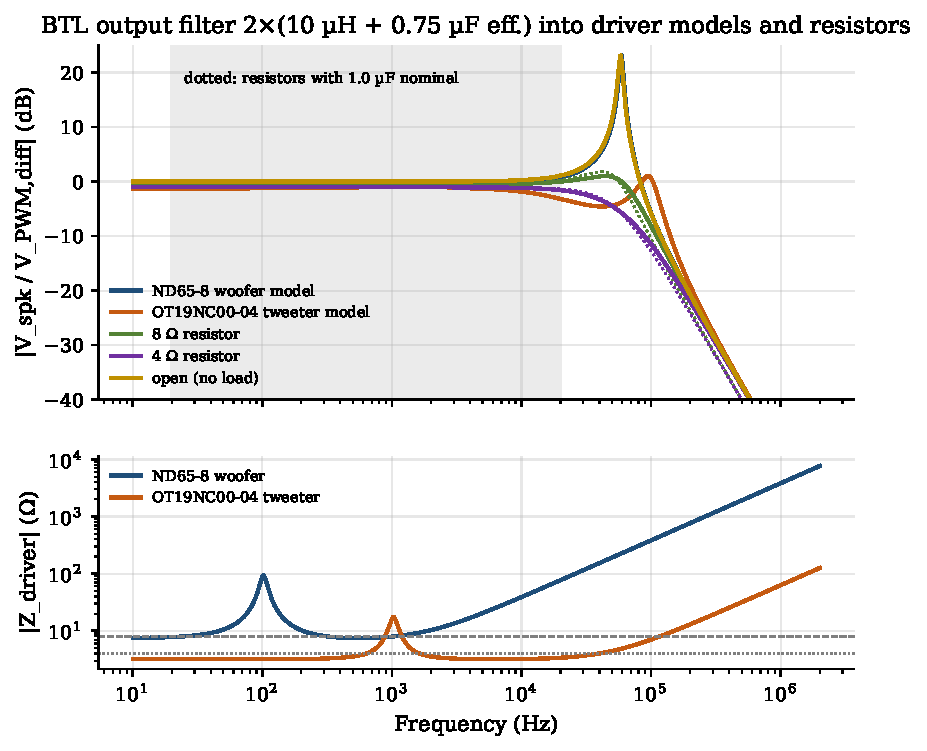
\includegraphics[width=\linewidth]{s2_filter_response.pdf}\caption{Filter into the driver models and into resistors.}\end{subfigure}\hfill
\begin{subfigure}[t]{0.49\linewidth}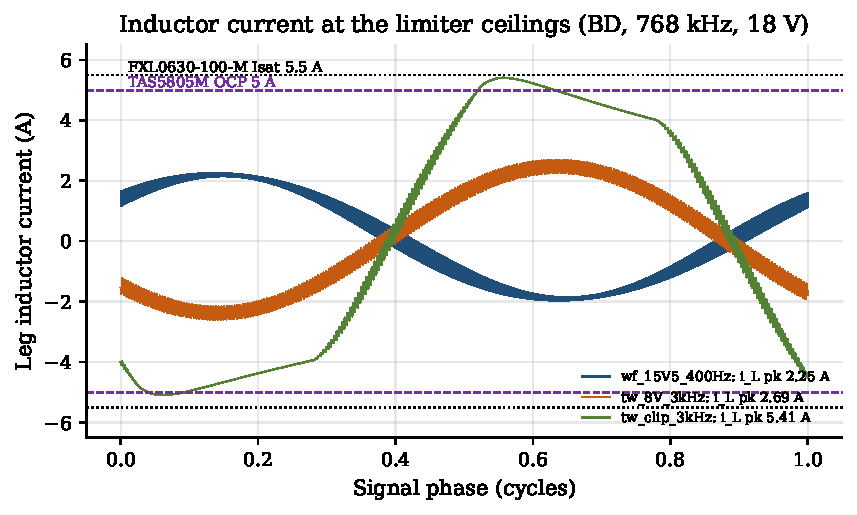
\includegraphics[width=\linewidth]{s2_inductor_peaks.pdf}\caption{Peak inductor current at the limiter ceilings and with a clipped tweeter.}\par\medskip
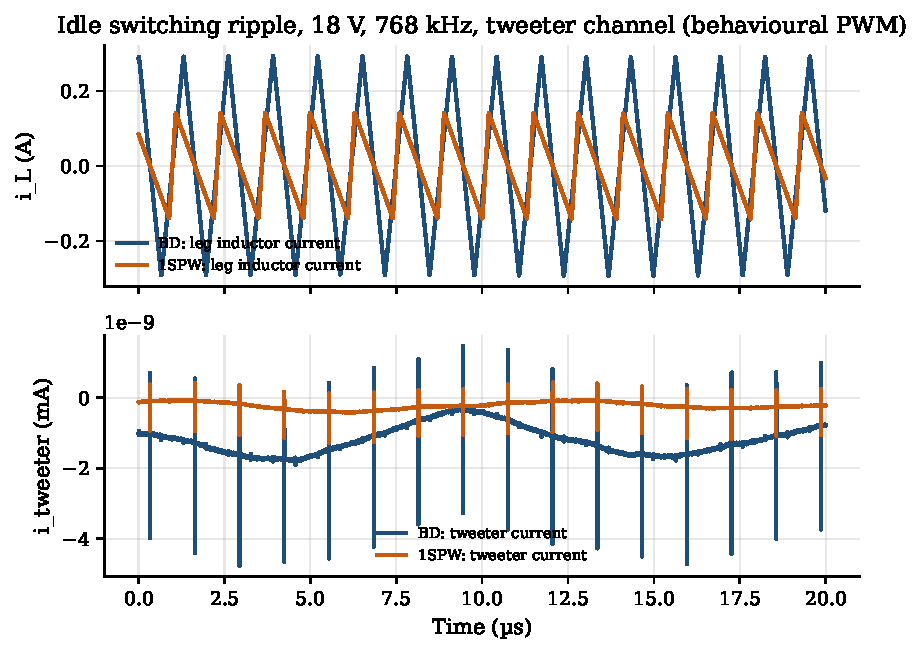
\includegraphics[width=\linewidth]{s2_idle_ripple.pdf}\caption{Idle ripple circulates in the filter capacitors, not the drivers.}\end{subfigure}
\caption{S2: a loudspeaker is not a resistor.}
\label{fig:s2}
\end{figure}

\subsubsection{S3--S5: NTC window, PVDD trim, ESP32 reset}\label{sec:s3}\label{sec:s4}\label{sec:s5}

\begin{itemize}
  \item \textbf{S3, NTC.} The charge window is \qtyrange{2.0}{60.8}{\degreeCelsius}, and an open NTC fails safe. With the charger's defaults it would keep charging from 45 to \qty{61}{\degreeCelsius}, so firmware stops it at \qty{45}{\degreeCelsius} (ECO-001 \#6).
  \item \textbf{S4, trim.} PVDD trims from \qty{18.0}{\volt} down to \qty{12.2}{\volt}. The curve sits \qty{0.3}{\volt} below the hand table, because the diode drops \qty{0.35}{\volt} at microamps, not \qty{0.45}{\volt}. It settles in \qtyrange{70}{110}{\milli\second}, and PWM ripple at the feedback node is below \qty{0.5}{\micro\volt}.
  \item \textbf{S5, reset.} With \qty{1}{\micro\farad}, esptool's auto-reset fails if the host leaves more than about \qty{2.5}{\milli\second} between its DTR and RTS requests. \qty{2.2}{\micro\farad} doubles the tolerance to \qty{5}{\milli\second} and also stops EN rising before the rail is valid (ECO-001 \#4). All strap levels read correctly.
\end{itemize}

\begin{figure}[htbp]
\centering
\begin{subfigure}[t]{0.49\linewidth}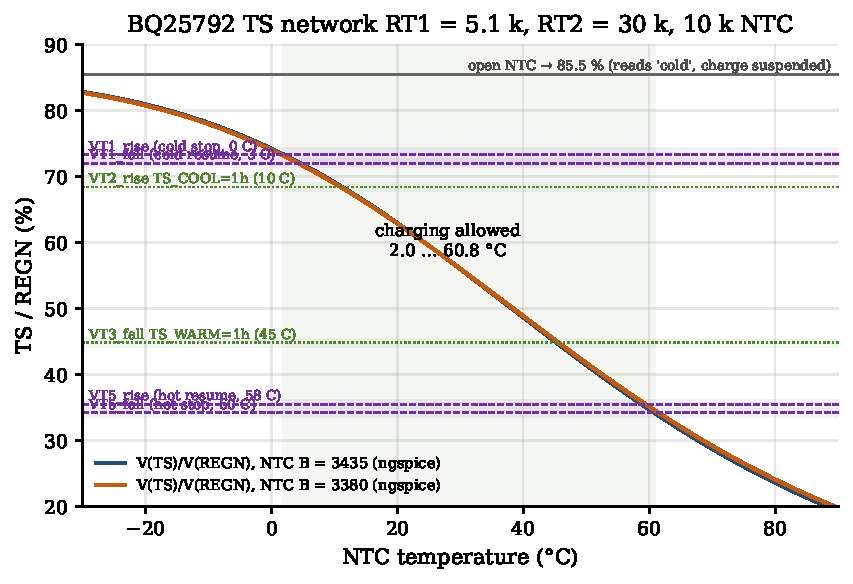
\includegraphics[width=\linewidth]{s3_ntc_window.pdf}\caption{S3: TS/REGN against temperature with the charger's thresholds.}\end{subfigure}\hfill
\begin{subfigure}[t]{0.49\linewidth}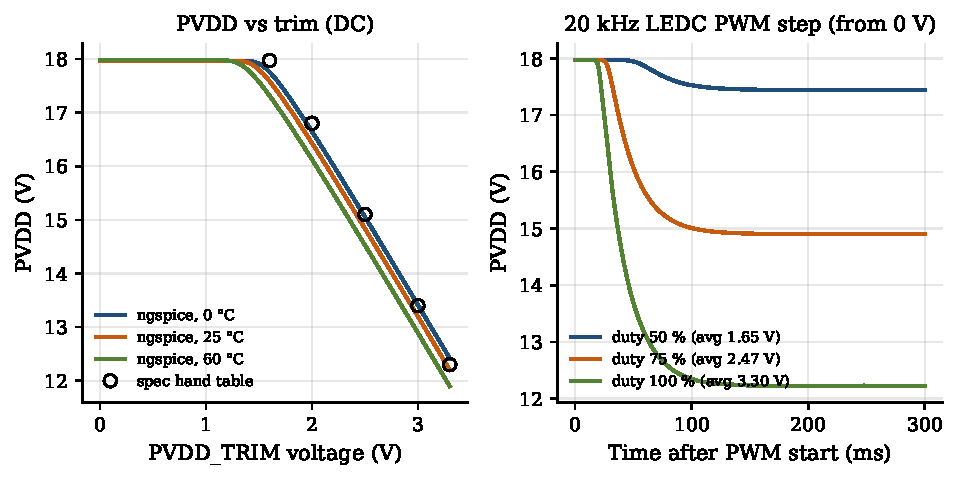
\includegraphics[width=\linewidth]{s4_pvdd_trim.pdf}\caption{S4: PVDD against trim voltage, and PWM transients.}\end{subfigure}\\[4pt]
\begin{subfigure}[t]{0.49\linewidth}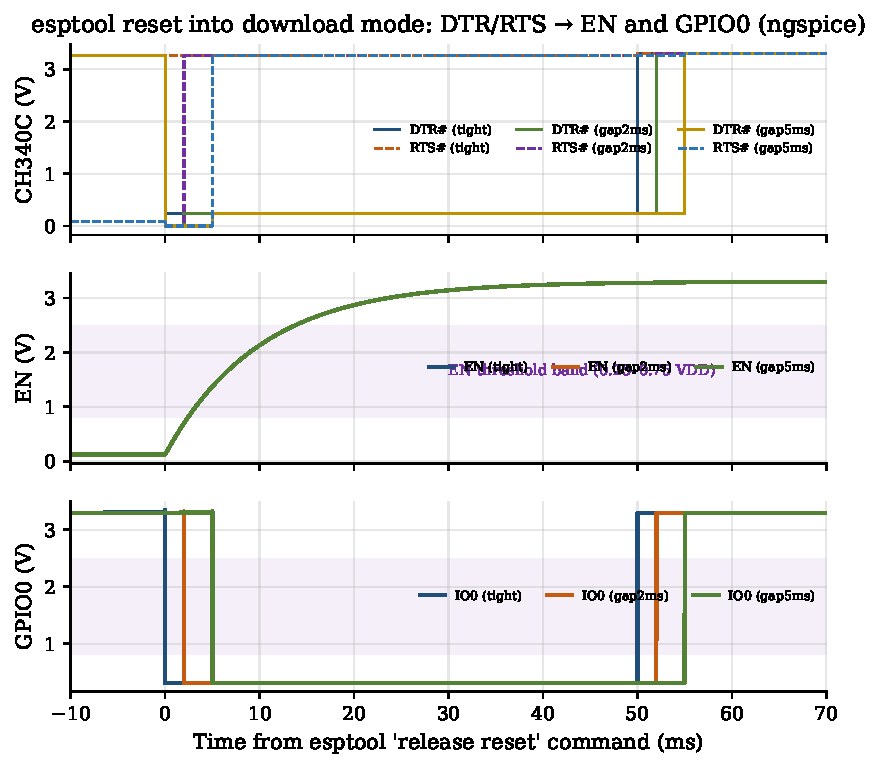
\includegraphics[width=\linewidth]{s5_autoreset.pdf}\caption{S5: auto-reset for the tight sequence and \qtylist{2;5}{\milli\second} gaps.}\end{subfigure}\hfill
\begin{subfigure}[t]{0.49\linewidth}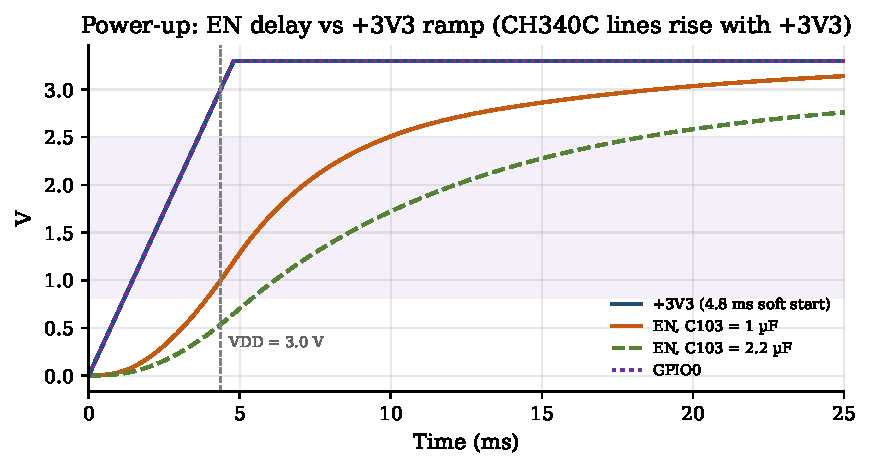
\includegraphics[width=\linewidth]{s5_powerup.pdf}\caption{S5: power-up with \qty{1}{\micro\farad} against \qty{2.2}{\micro\farad}.}\end{subfigure}
\caption{S3--S5: small circuits with real consequences.}
\label{fig:s3s5}
\end{figure}

\subsubsection{S6: Signal integrity on the UI flat cable}\label{sec:s6}

A 2-D field solver gives the 20-way FFC with ground on both sides of the clock as a $\approx\qty{107}{\ohm}$ line, twice what the ``\qty{33}{\ohm} for \qty{50}{\ohm}'' rule of thumb assumes. With \qty{33}{\ohm} source resistors, SCLK at \qty{40}{\mega\hertz} overshoots by \qtyrange{0.7}{1.1}{\volt}, enough to conduct the receiver's ESD diodes. With \qty{68}{\ohm} the overshoot is \qty{0.2}{\volt} at worst, and the clock can safely reach \qty{53}{\mega\hertz} (ECO-001 \#3). Crosstalk stays below the input-low threshold. The simulation used a \qty{200}{\milli\metre} cable; the build uses \qty{100}{\milli\metre}, so the results are conservative.

\begin{figure}[htbp]
\centering
\begin{subfigure}[t]{0.49\linewidth}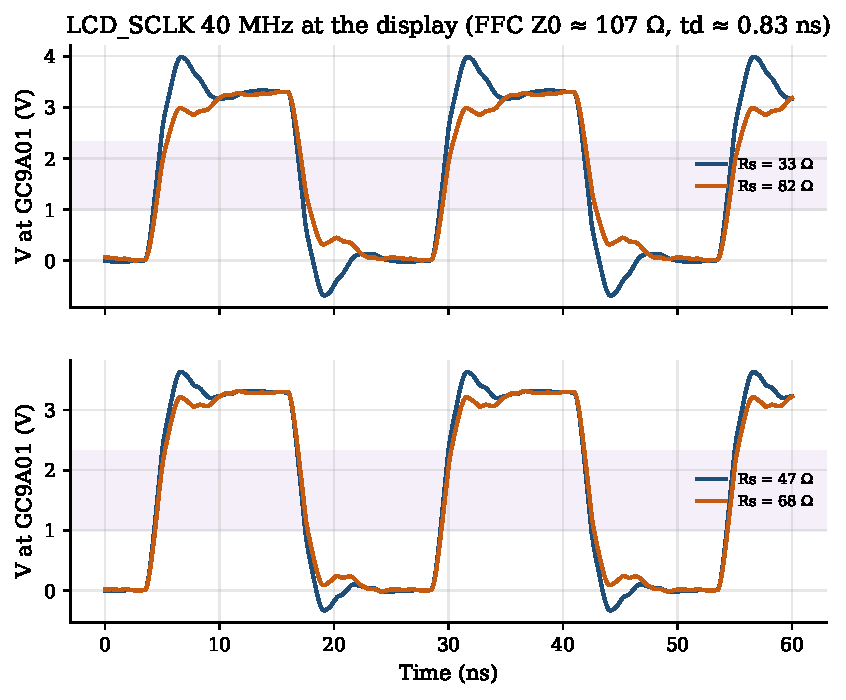
\includegraphics[width=\linewidth]{s6_sclk_40MHz.pdf}\caption{SCLK at the display for 33--\qty{82}{\ohm}.}\end{subfigure}\hfill
\begin{subfigure}[t]{0.49\linewidth}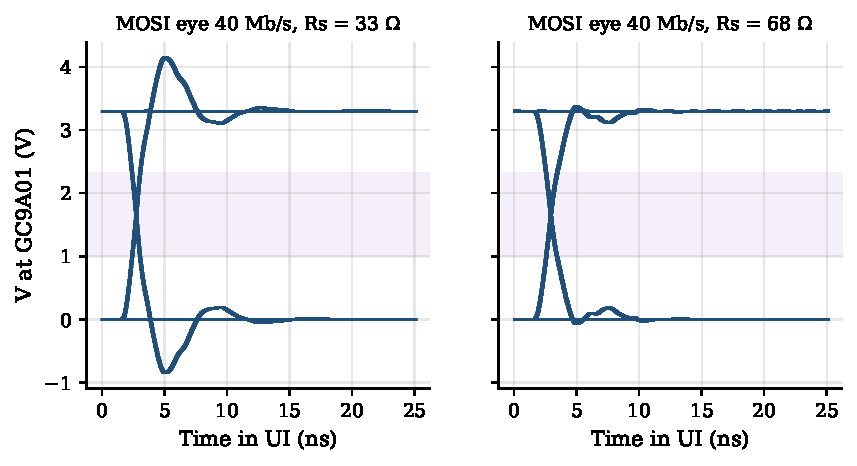
\includegraphics[width=\linewidth]{s6_mosi_eye.pdf}\caption{MOSI eye at \qty{40}{\mega\bit\per\second}, \qty{33}{\ohm} against \qty{68}{\ohm}.}\end{subfigure}\\[4pt]
\begin{subfigure}[t]{0.49\linewidth}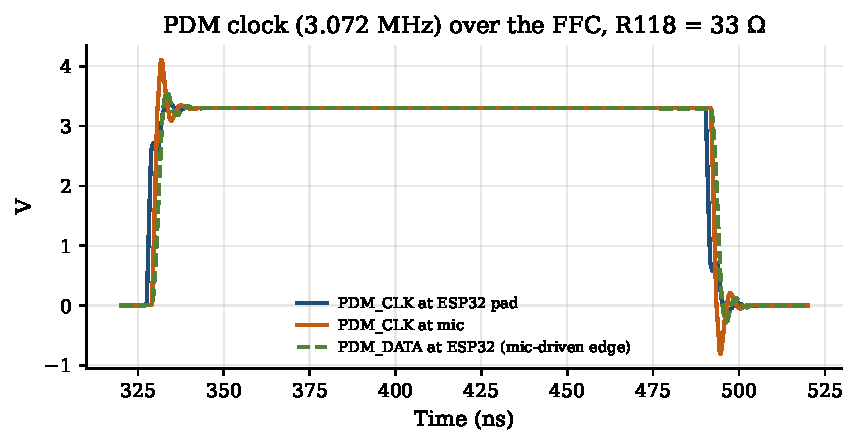
\includegraphics[width=\linewidth]{s6_pdm.pdf}\caption{PDM clock and the returning data edge.}\end{subfigure}\hfill
\begin{subfigure}[t]{0.49\linewidth}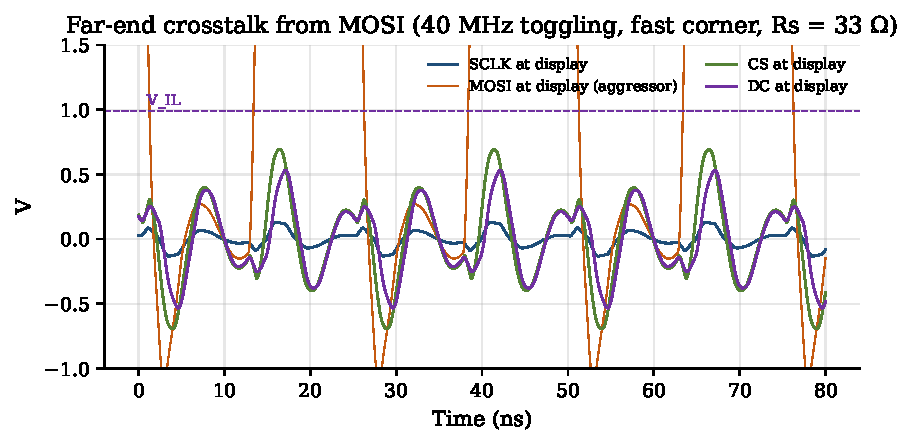
\includegraphics[width=\linewidth]{s6_crosstalk.pdf}\caption{Far-end crosstalk with MOSI toggling.}\end{subfigure}
\caption{S6: a ribbon cable is a transmission line.}
\label{fig:s6}
\end{figure}

\begin{checked}
\begin{itemize}[leftmargin=1.2em,itemsep=1pt]
  \item \textbf{S1:} hand crossover \qty{228}{\hertz} against \qty{247}{\hertz} modelled; hand impedance peak \qty{0.44}{\ohm} against \qty{0.46}{\ohm}. The averaged and switching models agree in shape; the switching model dips $1.6\times$ deeper because the error amplifier is slew-limited.
  \item \textbf{S2:} filter corner (\qty{50.3}{\kilo\hertz}) and idle ripple (\qty{0.585}{\ampere} against \qty{0.586}{\ampere}) match hand calculation.
  \item \textbf{S3:} TI's reference network is reproduced within 0.5 percentage points of REGN.
  \item \textbf{S6:} the field solver matches conformal mapping within \qty{0.1}{\percent}.
  \item \textbf{S7:} the PVDD peak matches the hand value.
  \item \textbf{Not done:} the injection loop-gain measurement and one load-step corner stalled in ngspice and were dropped. Both moved to the bench list.
\end{itemize}
\end{checked}
\FloatBarrier
